\documentclass[
    twocolumn,
    fontsize = 10pt,
    parskip = half+,
    headings = small,
    headwidth = text,
    footwidth = text,
]{scrartcl}

% --- KOMA-Script Settings ---
\KOMAoptions{
    paper = A4,
    pagesize,
    DIV = calc,
}
\typearea{11}

% --- Graphics ---
\usepackage{pdflscape}
\usepackage{pgfgantt}
\usepackage{pdflscape}
\usetikzlibrary{shapes,backgrounds, arrows, positioning, trees, shadows}
\usepackage{graphicx}  % make sure this is in your preamble
\usepackage{caption}   % for \captionof
\usepackage{comment}

% --- Math and Units ---
\usepackage{amsmath}
\usepackage[detect-all]{siunitx}

% --- Citations and Bibliography ---
\usepackage[style=ieee, backend=biber]{biblatex}
\addbibresource{bib/bibliography.bib}

% --- Links and Cross-Referencing ---
\usepackage{xurl}
\usepackage[colorlinks=true, allcolors=]{hyperref}
\usepackage[capitalize, nameinlink, noabbrev]{cleveref}

% --- Document Metadata ---
\title{Name of the project}
\subtitle{Floatsat 2025/2026}
\author{Mert Yigit Ozkan (TL/Mechanical Design),\\
        Jonas Schmidt (Mechanical Design),\\
        Shridevi S. Keraklamatti (Mechanical Design),\\
        Abdirakhman Onabek (Control Design),\\
        Jan Luis Holtman (Electrical Design),\\
        Tymoteusz Burak (Software Design)}

\begin{document}
\twocolumn[
\begin{@twocolumnfalse}

\maketitle

\begin{abstract}
Following the title, the abstract is the \textbf{second} most frequently read part of a scientific report.
It informs about the general content and determines the report's relevance for the reader.
It is good practice to write the abstract when writing the report is \textbf{finished} in a way that it condenses and summarizes the content of the report.
Only start writing the abstract when all required research and work have been finished.
Make the abstract one paragraph without reference and use about \numrange{100}{300} words.
Be sure to only draw conclusions and make only statements that are included in the report.
Keep the text of the abstract in present tense.
A good approach to drafting an abstract is to start by summarizing each section of the report in \numrange{1}{2} sentences.
\end{abstract}
\end{@twocolumnfalse}
]

%\tableofcontents
\newpage

%+++++++++++++++++++++++++++++++++++++++++++++++++++++++++++++++++++++++++++++++
%+++++++++++++++++++++++++++++++++++++++++++++++++++++++++++++++++++++++++++++++


%------------------------------------------------------------------------------
\section{Introduction}
%------------------------------------------------------------------------------
The FloatSat project, conducted under the Chair of Space Informatics and Satellite Systems (SISAT) at Julius-Maximilians-Universität Würzburg, constitutes a comprehensive practical exercise in the design, development, and operation of spacecraft subsystems. The primary technical objective is the creation of a fully functional satellite prototype capable of three-degree-of-freedom attitude determination and control in a terrestrial environment. To emulate the dynamics of orbital flight, the system operates on a Spherical Air Bearing Unit (SABU), which provides a near-frictionless platform replicating the torque-free conditions of space.

The project is inherently multidisciplinary, integrating mechanical engineering, embedded electronics, and control theory to develop a system capable of accurate reference trajectory tracking and stable attitude control. To ensure structured development and traceability, the project follows a Systems Engineering framework, organized into seven strategic Work Packages (WPs). These WPs encompass the full development lifecycle, from requirements analysis and state-of-the-art review to mechanical and electrical subsystem design, control strategy evaluation, and software system integration.

The Preliminary Design Review (PDR) Report marks a pivotal milestone, offering an opportunity to evaluate the technical feasibility, system architecture, and readiness of the FloatSat prototype. This review establishes a validated foundation for subsequent optimization, integration, and performance testing, in which the system will be assessed against key metrics such as settling time, overshoot, and control effort.

The following sections present a comprehensive overview of the FloatSat design at the PDR stage, detailing the project scope, design methodology, subsystem specifications, and the rationale behind the proposed system architecture.\\
\begin{figure}[h]
    \centering
    \includegraphics[width=0.7\linewidth]{img/Patch.png}
    \caption{The mission patch of Team 4 FloatSat Project}
    \label{fig:placeholder}
\end{figure}
%------------------------------------------------------------------------------
\section{Preliminary Design Overview}
%------------------------------------------------------------------------------

%-----------------------------------------
%--\subsection{Requirements}
%-----------------------------------------
%--
%-----------------------------------------
\subsection{Mechanical Design}
%-----------------------------------------

\subsubsection{Requirements}
\paragraph{Functional Requirements}

\begin{itemize}
    \item The assembly shall allow the flywheel to rotate about an axis that goes through the point of rotation.
    \item The assembly shall provide mounting locations for all required electronic boards.
    \item The base plate shall be expandable so that additional components can be added later (e.g., extra mounting holes or a grid pattern).
    \item The accelerometer shall be placed as close as practical to the rotational center in the plane of rotation.
    \item The design shall include features to fine-tune the center of mass in the \(x\!x\) plane (e.g., adjustable).
    \item The design shall provide paths, holes, or slots for cable routing and attachment of cable ties.
    \item All screws and fasteners shall be accessible with standard tools without removing unrelated parts.
\end{itemize}

\paragraph{Performance Requirements}

\begin{itemize}
    \item The axis of flywheel rotation shall be aligned with the geometric rotational center of the assembly.
    \item The center of mass of the complete assembly shall lie as close as reasonable along the \(z\) rotation axis; it may be lower in the \(x\) axis.
    \item The overall height of the assembly shall be kept as low as practical.
    \item The design shall minimize the number of separate parts while still meeting all other requirements.
    \item The design shall minimize the total 3D-printed material volume while maintaining sufficient stiffness and strength.
\end{itemize}

\paragraph{Constraints}

\begin{itemize}
    \item Every structural part of the assembly shall be manufacturable with common 3D-printing processes (no unprintable overhangs or trapped volumes).
    \item The assembled parts shall fit within the build volume of a typical desktop 3D printer.
    \item The geometry shall include dedicated holes or features for cable management and zip-ties.
    \item The geometry shall not obstruct tool access to screws and connectors.
    \item All screws and inserts shall fit the M2 or M3 standard.
    \item The battery shall be easily accessible and removable.
\end{itemize}



\begin{comment}
The selected RWA configuration employs a triad of mutually orthogonal reaction wheels mounted within a single assembly that is intentionally tilted with respect to the spacecraft's body-fixed reference frame. This architectural decision represents a systems-level optimization to satisfy two critical mission constraints: precise center-of-gravity (CoG) management and robust fault tolerance. The primary rationale for this orientation is to co-locate the collective CoG of the RWA—comprising the system's most massive components—with both the central axis and uppermost plane of the hemispherical bus. This precise CoG placement is fundamental to the vehicle's dynamic stability; a CoG deviation from this optimized position would result in mechanical interference between the rotating structure and the containment cover during attitude maneuvers, generating destabilizing frictional torques that would exceed the system's control authority. The tilted orthogonal configuration achieves this essential mass property without requiring structurally inefficient, asymmetric support members that would introduce unwanted flexure and parasitic mass.

From a operational reliability perspective, this configuration provides enhanced functional redundancy compared to a conventional body-aligned orthogonal arrangement. The strategic tilt ensures that no single wheel's spin axis is parallel to any principal spacecraft axis, thereby eliminating single-point failures. In the event of any one wheel failure, the remaining two actuators maintain torque projection capability about all three body axes, enabling graceful degradation to a reduced-performance mode rather than complete loss of attitude control about a critical axis. This fault-tolerant characteristic is paramount for mission success given the absence of a fourth redundant wheel. Additionally, this consolidated assembly minimizes products of inertia, reducing dynamic cross-coupling between axes and simplifying control law formulation. The configuration thus represents an optimal synthesis of mass property control, structural efficiency, and operational reliability for the Floatsat mission profile.

\end{comment}

The assembly contains three flywheels, one for each rotational degree of freedom. Each flywheel is mounted orthogonally to the others, but the entire system is additionally rotated in two axes by 45° to optimize the center of gravity alignment along the global Z-axis. This geometric offset ensures that the effective axis of rotation of each flywheel passes directly through the system’s center of rotation, minimizing induced torques and improving control authority.

\begin{figure}[h]
    \centering
    \includegraphics[width=0.7\linewidth]{img/axis_of_rotation_center.jpeg}
    \caption{Axis of wheel rotation going trough center of rotation}
    \label{fig:axis_of_roation}
\end{figure}
To support the electronics, a compact multi-board stack is mounted above the flywheel plane. All PCBs are arranged such that connectors, test points, and fastening screws remain fully accessible. The accelerometer is positioned as close as physically possible to the geometric center of rotation, reducing measurement errors caused by centrifugal or tangential acceleration components.

Additionally the battery was chosen to be able to sit at different points to tune the center of gravity along the y axis, because the upper housing is non symmetric with respect to the y axis.

The base plate serves as the structural foundation of the assembly. It is designed to be modular and expandable, providing additional mounting points . Cable routing channels and tie-down features are integrated directly into the geometry to prevent wire interference with the rotating components.

All structural components are optimized for common FDM 3D-printing processes, avoiding unprintable overhangs and trapped geometries. The form factor remains within the constraints of a standard desktop printer build volume. All fasteners follow M2 or M3 standards, and the battery remains easily accessible and removable without disturbing other components.

\begin{figure}[h]
    \centering
    \includegraphics[width=0.7\linewidth]{img/top_profile.jpeg}
    \includegraphics[width=0.7\linewidth]{img/side_profile.jpeg}
    \caption{Side and top profile of assembly}
    \label{fig:axis_of_roation}
\end{figure}

%-----------------------------------------
\subsection{Electrical Design}
%-----------------------------------------
\begin{figure}[h]
    \centering
    \includegraphics[width=1\linewidth]{img/FloatSatSchematic.pdf}
    \caption{FloatSat Schematic}
    \label{fig:FloatSatSchematic}
\end{figure}

\subsubsection{Electrical Requirements}

\paragraph{Functional}
\begin{enumerate}
    \item The Battery shall to connect to the Power Distribution board.
    \item The Power Distribution Board shall power the Main Control Unit.
    \item The Power Distribution Board shall power the IMU.
    \item The Power Distribution Board shall power the Communication Controller.
    \item The Power Distribution Board shall power the Motor Driver Board.
    \item The IMU shall communicate with the Main Control Unit.
    \item The Driver Board outputs shall control the Motor phases.
\end{enumerate}

\paragraph{Interface Requirements}
\begin{enumerate}
    \item Duplex Communication between the Communication Controller and the Main Control Unit shall be provided.
    \item The Main Control Unit shall control 3 Outputs per Motor on the Driver Board.
	\item The Main Control Unit shall be able to provide 3 different PWM signals to the driver.
    \item The Main Control Unit shall be able to commute each motor phase independently.
\end{enumerate}

\paragraph{Performance Requirements}
\begin{enumerate}
    \item Communication between the Communication Controller and the Main Control Unit shall provide enough Bandwidth for control commands and telemetry.
\end{enumerate}

\paragraph{Environmental Requirements}
\begin{enumerate}
    \item The Connections shall withstand the Vibrations of the Flotation Environment
\end{enumerate}

%-----------------------------------------
\subsection{Control System Design}
%-----------------------------------------
The FloatSat attitude control system uses three reaction wheels arranged in a tilted orthogonal configuration (see Mechanical Design section). We implement a classical PID-based attitude controller for preliminary testing.

\subsubsection{Torque Authority and Wheel Geometry}

To evaluate the control authority of the chosen geometry, we analyzed the singular values of the wheel-axis matrix $N$ for different tilt angles between each wheel axis and the body $Z$-axis. The singular values  $\sigma_i$ quantify the achievable torque in each principal direction, while the condition number indicates how evenly torque can be applied across all axes (low $\kappa$ preferred).

$$
\kappa = \frac{\sigma_{max}}{\sigma_{min}}
$$

\begin{figure}[h]
    \centering
    \includegraphics[width=0.7\linewidth]{img/condition_number_vs_tilt.png}
    \includegraphics[width=0.7\linewidth]{img/singular_values_vs_tilt.png}
    \caption{Torque Authority vs. Tilt Angle}
    \label{fig:torque_authority_vs_tilt}
\end{figure}

The mechanical design places the wheels so that two 45° rotations yield an effective tilt of 54.736° from the $Z$-axis. This corresponds well with the region where the condition number is near its minimum, meaning torque is well-distributed and the actuator geometry is close to orthogonal. Increasing the tilt would improve yaw authority but degrade roll/pitch authority, which might be beneficiary due to FloatSat dish geometry but we've chosen to keep the 54.736° angle towards the $Z$-axis.

This also gave insight on how small offsets between the actual CoG and the nominal wheel placement affects torque authority. As shown in \ref{fig:torque_authority_vs_tilt}, even millimeter-scale shifts slightly distort the wheel-axis matrix but do not significantly degrade the condition number. Larger offsets might produce noticeable asymmetry, motivating a later potential upgrade to sliding-mode control if needed.

The problem that comes with simulation for now is that we won't be able to know the exact inertia of our satellite body and flywheels. Thus we might implement a sliding control later that will counteract the unknown inertia of the sattelite or manually tune the PID so it's "good enough.

%-----------------------------------------
\subsection{Software System Design}
%-----------------------------------------
...

%------------------------------------------------------------------------------


%------------------------------------------------------------------------------
\section{Conclusion}
%------------------------------------------------------------------------------
In engineering and some other disciplines, the Conclusion is often integrated with the Discussion section.
Crafting the Conclusion:
\begin{itemize}
    \item Summarize Key Findings: Concisely restate the main findings of your research.
    \item Take-Home Message: Clearly articulate the core message or insight that you want readers to take away from your work. This should be a distillation of your
\end{itemize}
%\printbibliography
%\printglossaries
% Appendix
%\appendix
% \pagenumbering{roman}
%\include{appendix/appendix}
\onecolumn
\begin{landscape}
\section{Project Management}
%______________________________________________________________
% Work Breakdown Structure
% Breakdown of the tasks in individual work packages.
% Up to two levels of workpackages
%______________________________________________________________
\subsection{Work Breakdown Structure}
\scalebox{0.67}{
    \small
    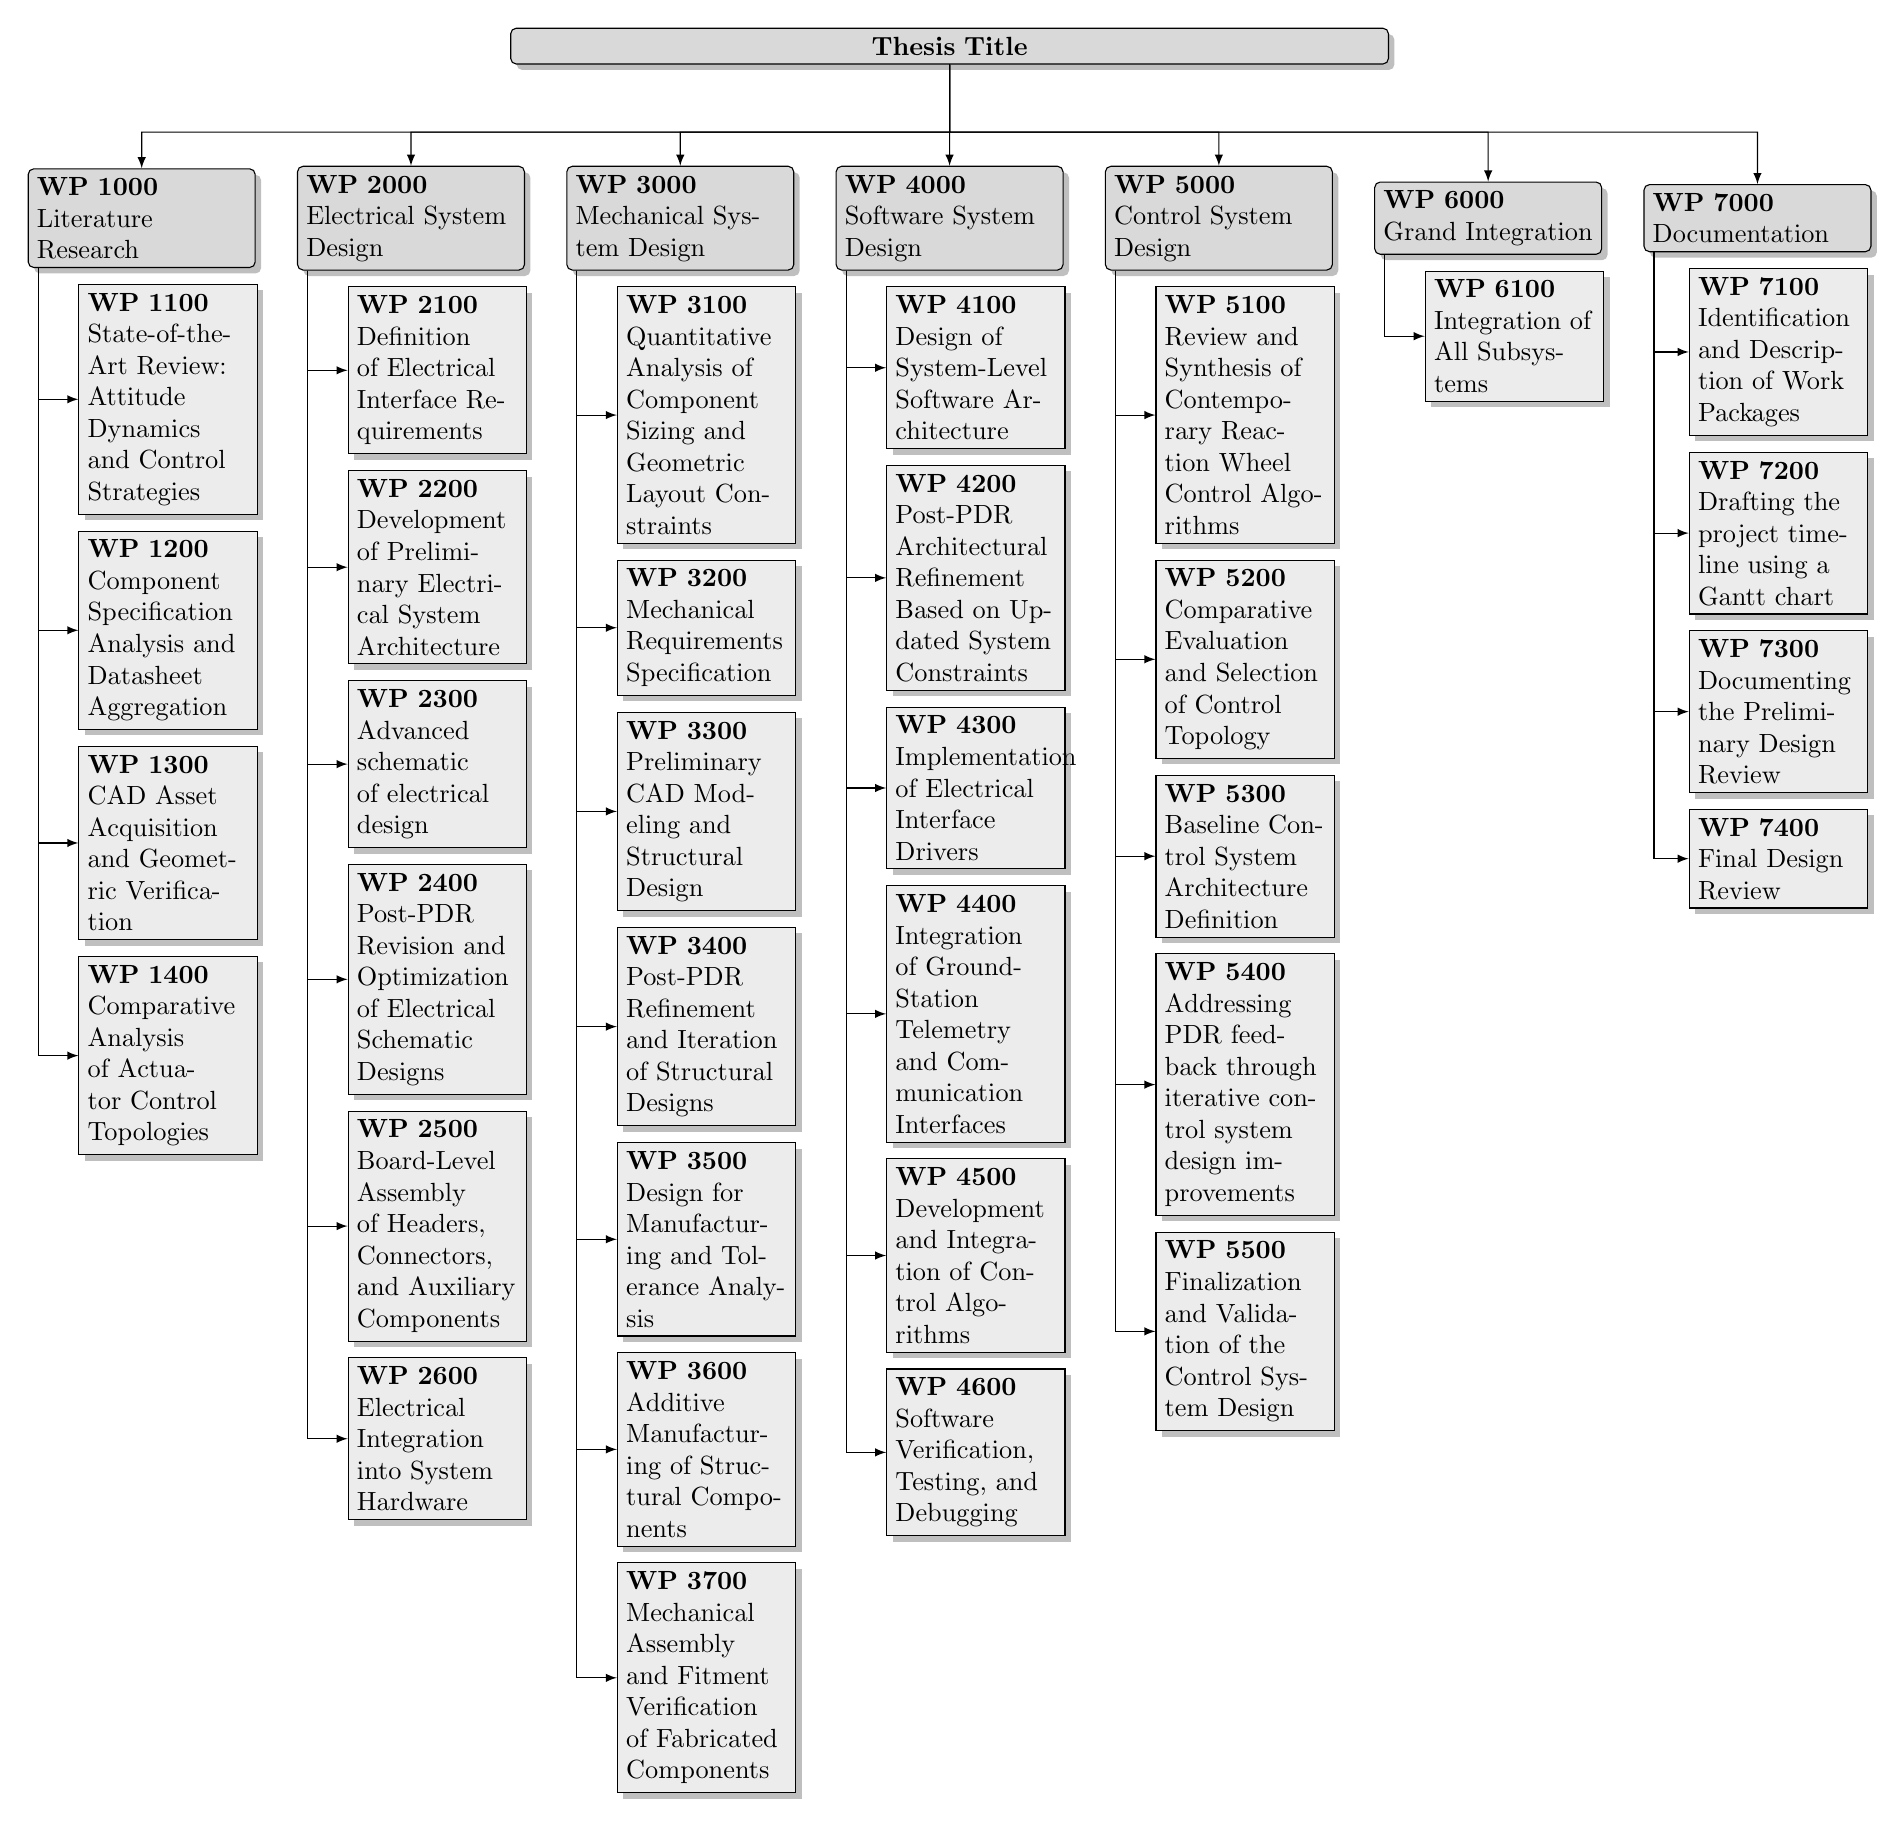
\begin{tikzpicture}[transform shape, scale=0.95,
        basic/.style   = {draw, text width=2.8cm, align=left, drop shadow, rectangle},
        root/.style    = {basic, text width=11.5cm, rounded corners=2pt, thin, align=center, fill=gray!30},
        level 2/.style = {basic, rounded corners=2pt, thin, fill=gray!30},
        level 3/.style = {basic, thin, fill=gray!15, text width=2.15cm},
        level 1/.style={sibling distance=36mm}, edge from parent fork down,
        edge from parent/.style={->,draw}, level distance=2.3cm,  >=latex]

        % root of the the initial tree, level 1
        \node[root] {\textbf{Thesis Title}}
        % The first level, as children of the initial tree
            child {node[level 2] (c1) {\textbf{WP~1000} \\ Literature\\ Research}}
            child {node[level 2] (c2) {\textbf{WP~2000} \\ Electrical System Design}}
            child {node[level 2] (c3) {\textbf{WP~3000} \\ Mechanical System Design}}
            child {node[level 2] (c4) {\textbf{WP~4000} \\ Software System Design}}
            child {node[level 2] (c5) {\textbf{WP~5000} \\ Control System \\Design}}
            child {node[level 2] (c6) {\textbf{WP~6000} \\ Grand Integration}}
            child {node[level 2] (c7) {\textbf{WP~7000} \\ Documentation}};
    
        % The second level, relatively positioned nodes
        \begin{scope}[every node/.style={level 3}, node distance=6pt]
            % WP 1000 children (converted from WP 1.x)
            \node [below=of c1, xshift=10pt] (c11) {\textbf{WP~1100} \\ State-of-the-Art Review: Attitude Dynamics and Control Strategies};
            \node [below=of c11] (c12) {\textbf{WP~1200} \\ Component Specification Analysis and Datasheet Aggregation};
            \node [below=of c12] (c13) {\textbf{WP~1300} \\ CAD Asset Acquisition and Geometric Verification};
            \node [below=of c13] (c14) {\textbf{WP~1400} \\ Comparative Analysis of Actuator Control Topologies};
            
            
            % WP 2000 children (converted from WP 2.x)
            \node [below=of c2, xshift=10pt] (c21) {\textbf{WP~2100} \\ Definition of Electrical Interface Requirements};
            \node [below=of c21] (c22) {\textbf{WP~2200} \\ Development of Preliminary Electrical System Architecture};
            \node [below=of c22] (c23) {\textbf{WP~2300} \\ Advanced schematic of electrical design};
            \node [below=of c23] (c24) {\textbf{WP~2400} \\ Post-PDR Revision and Optimization of Electrical Schematic Designs};
            \node [below=of c24] (c25) {\textbf{WP~2500} \\ Board-Level Assembly of Headers, Connectors, and Auxiliary Components};
            \node [below=of c25] (c26) {\textbf{WP~2600} \\ Electrical Integration into System Hardware};
            
            
            % WP 3000 children (converted from WP 3.x)
            \node [below=of c3, xshift=10pt] (c31) {\textbf{WP~3100} \\ Quantitative Analysis of Component Sizing and Geometric Layout Constraints};
            \node [below=of c31] (c32) {\textbf{WP~3200} \\ Mechanical Requirements Specification};
            \node [below=of c32] (c33) {\textbf{WP~3300} \\ Preliminary CAD Modeling and Structural Design};
            \node [below=of c33] (c34) {\textbf{WP~3400} \\ Post-PDR Refinement and Iteration of Structural Designs};
            \node [below=of c34] (c35) {\textbf{WP~3500} \\ Design for Manufacturing and Tolerance Analysis};
            \node [below=of c35] (c36) {\textbf{WP~3600} \\ Additive Manufacturing of Structural Components};
            \node [below=of c36] (c37) {\textbf{WP~3700} \\ Mechanical Assembly and Fitment Verification of Fabricated Components};
            
            
            % WP 4000 children (converted from WP 4.x)
            \node [below=of c4, xshift=10pt] (c41) {\textbf{WP~4100} \\ Design of System-Level Software Architecture};
            \node [below=of c41] (c42) {\textbf{WP~4200} \\ Post-PDR Architectural Refinement Based on Updated System Constraints};
            \node [below=of c42] (c43) {\textbf{WP~4300} \\ Implementation of Electrical Interface Drivers};
            \node [below=of c43] (c44) {\textbf{WP~4400} \\ Integration of Ground-Station Telemetry and Communication Interfaces};
            \node [below=of c44] (c45) {\textbf{WP~4500} \\ Development and Integration of Control Algorithms};
            \node [below=of c45] (c46) {\textbf{WP~4600} \\ Software Verification, Testing, and Debugging};
            
            
            % WP 5000 children (converted from WP 5.x)
            \node [below=of c5, xshift=10pt] (c51) {\textbf{WP~5100} \\ Review and Synthesis of Contemporary Reaction Wheel Control Algorithms};
            \node [below=of c51] (c52) {\textbf{WP~5200} \\ Comparative Evaluation and Selection of Control Topology};
            \node [below=of c52] (c53) {\textbf{WP~5300} \\ Baseline Control System Architecture Definition};
            \node [below=of c53] (c54) {\textbf{WP~5400} \\ Addressing PDR feedback through iterative control system design improvements};
            \node [below=of c54] (c55) {\textbf{WP~5500} \\ Finalization and Validation of the Control System Design};
            
            
            % WP 6000 children
            \node [below=of c6, xshift=10pt] (c61) {\textbf{WP~6100} \\ Integration of All Subsystems};
            
            % WP 7000 children
            \node [below=of c7, xshift=8pt] (c71) {\textbf{WP~7100} \\ Identification and Description of Work Packages};
            \node [below=of c71] (c72) {\textbf{WP~7200} \\ Drafting the project timeline using a Gantt chart};
            \node [below=of c72] (c73) {\textbf{WP~7300} \\ Documenting the Preliminary Design Review};
            \node [below=of c73] (c74) {\textbf{WP~7400} \\ Final Design Review};
        
        \end{scope}
    
        % lines from each level 1 node to every one of its "children"
        \foreach \value in {1,2,3,4}
            \draw[->] ([xshift=4pt]c1.south west) |- (c1\value.west);
    
        \foreach \value in {1,2,3,4,5,6}
            \draw[->] ([xshift=4pt]c2.south west) |- (c2\value.west);
    
        \foreach \value in {1,2,3,4,5,6,7}
            \draw[->] ([xshift=4pt]c3.south west) |- (c3\value.west);
    
        \foreach \value in {1,2,3,4,5,6}
            \draw[->] ([xshift=4pt]c4.south west) |- (c4\value.west);
            
        \foreach \value in {1,2,3,4,5}
            \draw[->] ([xshift=4pt]c5.south west) |- (c5\value.west);
            
        \foreach \value in {1}
            \draw[->] ([xshift=4pt]c6.south west) |- (c6\value.west);
    
        \foreach \value in {1,2,3,4}
            \draw[->] ([xshift=4pt]c7.south west) |- (c7\value.west);  
      
    \end{tikzpicture}
}
\end{landscape}


% %______________________________________________________________
% Gantt Chart
% Time line of the project
% Shows duration and chronological structure for each 
%  workpackage and project milestones
%______________________________________________________________
\subsection{Gantt Chart}

\definecolor{color_bar}{RGB}{0, 63, 137}
\definecolor{color_group}{RGB}{0, 37, 82}

\begin{center}
    % Resizebox forces the content to fit the text width.
    % We create a chart that is natively 28cm wide (much wider than the page),
    % then shrink it down. This makes the text smaller but the bars longer.
    \noindent\resizebox{\textwidth}{!}{%
    \begin{ganttchart}[
        expand chart=31cm,           % <--- KEY CHANGE: Render wider than the page
        y unit chart=0.6cm,          % Taller rows to keep them readable when scaled down
        vgrid,
        hgrid,
        bar/.append style={fill=color_bar, draw=none},
        group/.append style={fill=color_group},
        group left shift=0,
        group right shift=0,
        group peaks tip position=0,
        group peaks height=.25,
        group top shift=0.25,
        bar top shift=-0.1,
        bar height=0.6,
        milestone top shift=-0.1,
        milestone/.append style={fill=yellow, xscale=0.5}]{1}{16}
        
        \gantttitle{Weeks}{16} \\
        \gantttitlelist{1,...,16}{1} \\
         
        \ganttgroup{WP 1: Literature Research}{3}{6} \\
        \ganttbar{WP 1.1: State-of-the-Art Review: Attitude Dynamics and Control Strategies}{3}{4} \\
        \ganttbar{WP 1.2: Component Specification Analysis and Datasheet Aggregation}{4}{5} \\
        \ganttbar{WP 1.3: CAD Asset Acquisition and Geometric Verification}{4}{5} \\
        \ganttbar{WP 1.4: Comparative Analysis of Actuator Control Topologies}{5}{6} \\
        \\
        \ganttgroup{WP 2: Electrical System Design}{4}{12} \\
        \ganttbar{WP 2.1: Definition of Electrical Interface Requirements}{4}{5} \\
        \ganttbar{WP 2.2: Development of Preliminary Electrical System Architecture}{4}{5} \\
        \ganttbar{WP 2.3: Advanced Schematic of Electrical Design}{6}{7} \\
        \ganttmilestone[yellow]{PDR}{7} \\
        \ganttbar{WP 2.4: Post-PDR Revision and Optimization of Electrical Schematic Designs}{7}{8} \\
        \ganttbar{WP 2.5: oard-Level Assembly of Headers, Connectors, and Auxiliary Components}{8}{12} \\
        \ganttbar{WP 2.6: Electrical Integration into System Hardware}{8}{12} \\
        \ganttmilestone[yellow]{Project Progress Presentation}{13} \\
        \ganttmilestone[yellow]{Final Review}{16} \\
        \\
        \ganttgroup{WP 3: Mechanical System Design}{4}{16} \\
        \ganttbar{WP 3.1: Quantitative Analysis of Component Sizing and Geometric Layout Constraints}{4}{5} \\
        \ganttbar{WP 3.2: Mechanical Requirements Specification}{4}{5} \\
        \ganttbar{WP 3.3: Preliminary CAD Modeling and Structural Design}{4}{6} \\
        \ganttmilestone[yellow]{PDR}{7} \\
        \ganttbar{WP 3.4: Post-PDR Refinement and Iteration of Structural Designs}{4}{9} \\
        \ganttbar{WP 3.5: Design for Manufacturing and Tolerance Analysis}{7}{10} \\
        \ganttbar{WP 3.6: Additive Manufacturing of Structural Components}{10}{13} \\
        \ganttbar{WP 3.7: Mechanical Assembly and Fitment Verification of Fabricated Components}{10}{16} \\
        \ganttmilestone[yellow]{Project Progress Presentation}{13} \\
        \ganttmilestone[yellow]{Final Review}{16} \\
        \\
        \ganttgroup{WP 4: Software System Design}{3}{16} \\
        \ganttbar{WP 4.1: Design of System-Level Software Architecture}{3}{7} \\
        \ganttmilestone[yellow]{PDR}{7} \\
        \ganttbar{WP 4.2: Post-PDR Architectural Refinement Based on Updated System Constraints}{7}{8} \\
        \ganttbar{WP 4.3: Implementation of Electrical Interface Drivers}{7}{9} \\
        \ganttbar{WP 4.4: Integration of Ground-Station Telemetry and Communication Interfaces}{8}{14} \\
        \ganttbar{WP 4.5: Development and Integration of Control Algorithms}{7}{14} \\
        \ganttbar{WP 4.6: Software Verification, Testing, and Debugging}{12}{16} \\
        \ganttmilestone[yellow]{Project Progress Presentation}{13} \\
        \ganttmilestone[yellow]{Final Review}{16} \\
        \\
        \ganttgroup{WP 5: Control System Design}{3}{16} \\
        \ganttbar{WP 5.1: Review and Synthesis of Contemporary Reaction Wheel Control Algorithms}{3}{5} \\
        \ganttbar{WP 5.2: Comparative Evaluation and Selection of Control Topology}{4}{5} \\
        \ganttbar{WP 5.3: Baseline Control System Architecture Definition}{6}{8} \\
        \ganttmilestone[yellow]{PDR}{7} \\
        \ganttbar{WP 5.4: Addressing PDR feedback through iterative control system design improvements}{8}{9} \\
        \ganttbar{WP 5.5: Finalization and Validation of the Control System Design}{9}{16} \\
        \ganttmilestone[yellow]{Project Progress Presentation}{13} \\
        \ganttmilestone[yellow]{Final Review}{16} \\
        \\
        \ganttgroup{WP 6: Ground Integration}{8}{15} \\
        \ganttbar{WP 6.1: Integration of All Subsystems}{8}{15} \\
        \ganttmilestone[yellow]{Project Progress Presentation}{13} \\
        \ganttmilestone[yellow]{Final Review}{16}
        \\
        \ganttgroup{WP 7: Documentation}{3}{15} \\
        \ganttbar{WP 7.1: Identification and Description of Work Packages}{3}{4} \\
        \ganttbar{WP 7.2: Drafting the project timeline using a Gantt chart}{3}{4} \\
        \ganttbar{WP 7.3: Documenting the Preliminary Design Review}{4}{7} \\
        \ganttmilestone[yellow]{PDR}{7} \\
        \ganttbar{WP 7.4: Final Design Review}{12}{15} \\
        \ganttmilestone[yellow]{Final Review}{16}
    \end{ganttchart}
    }
\end{center}

\clearpage

%______________________________________________________________
% Work Package Description
% Detailed description of each workpackage
%______________________________________________________________

\subsection{Work Package Description}

\newcommand{\wpddate}{27.10.2025}
%%%%
% WP1000 - Literature Research
%%%%

\begin{table}[h!]
\centering
\scalebox{0.48}{  % change the variable in order to scale the table
\begin{tabular}{c c}

% --- WP1100 ---
\begin{tabular}{|p{.2\columnwidth}||p{.3\columnwidth}|p{.27\columnwidth}||p{.23\columnwidth}|}
    \hline
    \multicolumn{3}{|l||}{\textbf{}} & \multicolumn{1}{c|}{\textbf{WP 1100}}\\
    \hline\hline
    \textbf{Title} & \multicolumn{2}{p{.40\columnwidth}||}{\textbf{State-of-the-Art Review: Attitude Dynamics and Control Strategies}}
    & \textbf{Version:} 1.0\\
    \hline
    \textbf{Responsible} & \multicolumn{2}{l||}{Abdirakhman Onabek}
    & \textbf{Date:} \wpddate\\
    \hline\hline
    \textbf{Start - End} & \multicolumn{2}{l||}{Week 3 - Week 4}
    & \textbf{Duration}: 1 Week\\
    \hline
    \textbf{Processed by} & \multicolumn{3}{l|}{ALL}\\
    \hline\hline
    \multicolumn{4}{|p{.95\columnwidth}|}{\textbf{Goals:}}\\
    \multicolumn{4}{|p{.95\columnwidth}|}{$\bullet$ The primary objective is to establish a robust theoretical baseline for the project, ensuring that the chosen control strategies are both technically feasible and aligned with the project's time constraints. This involves defining the specific mathematical frameworks for attitude dynamics to prevent scope creep and setting clear acceptance criteria for system stability and performance.}\\
    \multicolumn{4}{|p{.95\columnwidth}|}{}\\
    \multicolumn{4}{|p{.95\columnwidth}|}{\textbf{Input:}}\\
    \multicolumn{4}{|p{.95\columnwidth}|}{$\bullet$ The work is grounded in the initial thesis scope definition and supported by access to established aerospace research resources. This includes the use of standard scholarly databases—such as IEEE Xplore and the AIAA Digital Library—as well as authoritative academic textbooks covering spacecraft dynamics, control, and related foundational principles.}\\
    \multicolumn{4}{|p{.95\columnwidth}|}{}\\
    \multicolumn{4}{|p{.95\columnwidth}|}{\textbf{Connections to other WPs:}}\\
    \multicolumn{4}{|p{.95\columnwidth}|}{$\bullet$ This package lies on the critical path for WP 5300, as the mathematical models derived here define the physics engine for the simulation, and it sets the computational complexity constraints that guide the software system design in WP 4000.}\\    
    \multicolumn{4}{|p{.95\columnwidth}|}{\textbf{Tasks:}}\\
    \multicolumn{4}{|p{.95\columnwidth}|}{$\bullet$ Conducting a comprehensive literature search to categorize control strategies into basic and advanced tiers, followed by a trade-off analysis to identify the most viable approach based on complexity versus performance. The resulting insights will be synthesized into the literature review chapter, forming the project’s theoretical foundation and supporting the rationale behind the selected design choices.}\\
    \multicolumn{4}{|p{.95\columnwidth}|}{}\\
    \multicolumn{4}{|p{.95\columnwidth}|}{\textbf{Results:}}\\
    \multicolumn{4}{|p{.95\columnwidth}|}{$\bullet$ The output consists of a structured synthesis of relevant research and a formal decision on the mathematical model to be adopted. This outcome establishes the project’s analytical foundation and acts as a key decision gate for the following design stages.}\\
    \hline
\end{tabular}
&
% --- WP1200 ---
\begin{tabular}{|p{.2\columnwidth}||p{.3\columnwidth}|p{.27\columnwidth}||p{.23\columnwidth}|}
    \hline
    \multicolumn{3}{|l||}{\textbf{}} & \multicolumn{1}{c|}{\textbf{WP 1200}}\\
    \hline\hline
    \textbf{Title} & \multicolumn{2}{p{.40\columnwidth}||}{\textbf{Component Specification Analysis and Datasheet Aggregation}}
    & \textbf{Version:} 1.0\\
    \hline
    \textbf{Responsible} & \multicolumn{2}{l||}{Abdirakhman Onabek}
    & \textbf{Date:} \wpddate\\
    \hline\hline
    \textbf{Start - End} & \multicolumn{2}{l||}{Week 4  - Week 5}
    & \textbf{Duration}: 1.5 Weeks\\
    \hline
    \textbf{Processed by} & \multicolumn{3}{l|}{Abdirakhman Onabek, Jan Luis Holtman, Tymoteusz Burak}\\
    \hline\hline
    \multicolumn{4}{|p{.95\columnwidth}|}{\textbf{Goals:}}\\
    \multicolumn{4}{|p{.95\columnwidth}|}{$\bullet$ The aim of this work is to collect component datasheets and review them to make sure each part meets the project requirements.}\\
    \multicolumn{4}{|p{.95\columnwidth}|}{}\\
    \multicolumn{4}{|p{.95\columnwidth}|}{\textbf{Input:}}\\
    \multicolumn{4}{|p{.95\columnwidth}|}{$\bullet$ Inputs include the functional requirements specification from the initial research phase and the predefined component list provided by the laboratory.}\\
    \multicolumn{4}{|p{.95\columnwidth}|}{}\\
    \multicolumn{4}{|p{.95\columnwidth}|}{\textbf{Connections to other WPs:}}\\
    \multicolumn{4}{|p{.95\columnwidth}|}{This is a mandatory prerequisite for both the Electrical (WP 2100) and Mechanical (WP 3100) design phases, as physical and electrical interfaces cannot be designed without frozen component specifications.}\\
    \multicolumn{4}{|p{.95\columnwidth}|}{\textbf{Tasks:}}\\
    \multicolumn{4}{|p{.95\columnwidth}|}{$\bullet$ The work involves mapping each components to specific project requirements to avoid over-engineering, ensuring that all components—supplied by the laboratory—meet project needs, and creating a centralized, version-controlled repository for all technical documentation to guarantee team-wide access.}\\
    \multicolumn{4}{|p{.95\columnwidth}|}{}\\
    \multicolumn{4}{|p{.95\columnwidth}|}{\textbf{Results:}}\\
    \multicolumn{4}{|p{.95\columnwidth}|}{$\bullet$ The deliverables are well-organized digital library of corresponding datasheets ready for engineering use.}\\
    \hline
\end{tabular}

\end{tabular}
}
\end{table}

\begin{table}[h!]
\centering
\scalebox{0.48}{  % change the variable in order to scale the table
\begin{tabular}{c c}

% --- WP1300 ---
\begin{tabular}{|p{.2\columnwidth}||p{.3\columnwidth}|p{.27\columnwidth}||p{.23\columnwidth}|}
    \hline
    \multicolumn{3}{|l||}{\textbf{}} & \multicolumn{1}{c|}{\textbf{WP 1300}}\\
    \hline\hline
    \textbf{Title} & \multicolumn{2}{p{.40\columnwidth}||}{\textbf{CAD Asset Acquisition and Geometric Verification}}
    & \textbf{Version:} 1.0\\
    \hline
    \textbf{Responsible} & \multicolumn{2}{l||}{Jonas Schmidt}
    & \textbf{Date:} \wpddate\\
    \hline\hline
    \textbf{Start - End} & \multicolumn{2}{l||}{Week 4  - Week 5}
    & \textbf{Duration}: 1.5 Weeks\\
    \hline
    \textbf{Processed by} & \multicolumn{3}{l|}{Jonas Schmidt, Mert Yigit Ozkan, Shridevi S. Keraklamatti}\\
    \hline\hline
    \multicolumn{4}{|p{.95\columnwidth}|}{\textbf{Goals:}}\\
    \multicolumn{4}{|p{.95\columnwidth}|}{$\bullet$ Acquire accurate CAD models of all critical components and verify their geometric and mass properties.}\\
    \multicolumn{4}{|p{.95\columnwidth}|}{}\\
    \multicolumn{4}{|p{.95\columnwidth}|}{\textbf{Input:}}\\
    \multicolumn{4}{|p{.95\columnwidth}|}{$\bullet$ Manufacturer datasheets and CAD files for components.}\\
    \multicolumn{4}{|p{.95\columnwidth}|}{}\\
    \multicolumn{4}{|p{.95\columnwidth}|}{\textbf{Connections to other WPs:}}\\
    \multicolumn{4}{|p{.95\columnwidth}|}{Deliver the verified CAD models, mass properties, and standardized component library to WP 5300 for dynamics modeling, to WP 3000 for integration into the main satellite assembly design, and to WP 4500 to define placement constraints and interface geometries.}\\
    \multicolumn{4}{|p{.95\columnwidth}|}{\textbf{Tasks:}}\\
    \multicolumn{4}{|p{.95\columnwidth}|}{$\bullet$ Collect and organize all necessary CAD assets, verify each component’s dimensions, interfaces, and materials, extract and document accurate mass properties for dynamics modeling, and assemble a standardized STEP-format component library.}\\
    \multicolumn{4}{|p{.95\columnwidth}|}{}\\
    \multicolumn{4}{|p{.95\columnwidth}|}{\textbf{Results:}}\\
    \multicolumn{4}{|p{.95\columnwidth}|}{$\bullet$ The deliverable is a verified .STEP Component Library ready for import into the main assembly.}\\
    \hline
\end{tabular}
&
% --- WP1400 ---
\begin{tabular}{|p{.2\columnwidth}||p{.3\columnwidth}|p{.27\columnwidth}||p{.23\columnwidth}|}
    \hline
    \multicolumn{3}{|l||}{\textbf{}} & \multicolumn{1}{c|}{\textbf{WP 1400}}\\
    \hline\hline
    \textbf{Title} & \multicolumn{2}{p{.40\columnwidth}||}{\textbf{Comparative Analysis of Actuator Control Topologies}}
    & \textbf{Version:} 1.0\\
    \hline
    \textbf{Responsible} & \multicolumn{2}{l||}{Abdirakhman Onabek}
    & \textbf{Date:} \wpddate\\
    \hline\hline
    \textbf{Start - End} & \multicolumn{2}{l||}{Week 5  - Week 6}
    & \textbf{Duration}: 1.5 Weeks\\
    \hline
    \textbf{Processed by} & \multicolumn{3}{l|}{Abdirakhman Onabek, Jan Luis Holtman, Tymoteusz Burak}\\
    \hline\hline
    \multicolumn{4}{|p{.95\columnwidth}|}{\textbf{Goals:}}\\
    \multicolumn{4}{|p{.95\columnwidth}|}{$\bullet$ The objective is to make a definitive "Design Freeze" decision on the physical layout of the actuators to allow parallel workflows in electrical, control and mechanical subsystems to proceed. The goal is to select a baseline configuration that meets minimum requirements without introducing unnecessary implementation complexity.}\\
    \multicolumn{4}{|p{.95\columnwidth}|}{}\\
    \multicolumn{4}{|p{.95\columnwidth}|}{\textbf{Input:}}\\
    \multicolumn{4}{|p{.95\columnwidth}|}{$\bullet$ The decision is based on the component limitations identified in WP 1200 and the baseline control requirements established in WP 1100.}\\
    \multicolumn{4}{|p{.95\columnwidth}|}{}\\
    \multicolumn{4}{|p{.95\columnwidth}|}{\textbf{Connections to other WPs:}}\\
    \multicolumn{4}{|p{.95\columnwidth}|}{This decision acts as a central dependency that dictates the structural layout and mounting constraints for the Mechanical System (WP 3000), while simultaneously defining the complexity of the algorithms required for the Control System (WP 5000). It also firmly establishes the interface requirements for the Electrical System (WP 2000) and the driver logic for the Software team (WP 4000), ensuring all subsystems are aligned on a single architecture.}\\
    \multicolumn{4}{|p{.95\columnwidth}|}{\textbf{Tasks:}}\\
    \multicolumn{4}{|p{.95\columnwidth}|}{$\bullet$ The team will review the standard configuration options and select the appropriate approach that satisfies the project goals. The focus is on confirming feasibility and formally documenting the decision to prevent future changes to the components.}\\
    \multicolumn{4}{|p{.95\columnwidth}|}{}\\
    \multicolumn{4}{|p{.95\columnwidth}|}{\textbf{Results:}}\\
    \multicolumn{4}{|p{.95\columnwidth}|}{$\bullet$ The deliverable is a decision on the system architecture, providing a clear and fixed direction that unblocks the detailed design phases for both control and software.}\\
    \hline
\end{tabular}

\end{tabular}
}
\end{table}


\begin{table}[h!]
\centering
\scalebox{0.48}{  % change the variable in order to scale the table
\begin{tabular}{c c}

% --- WP2100 ---
\begin{tabular}{|p{.2\columnwidth}||p{.3\columnwidth}|p{.27\columnwidth}||p{.23\columnwidth}|}
    \hline
    \multicolumn{3}{|l||}{\textbf{}} & \multicolumn{1}{c|}{\textbf{WP 2100}}\\
    \hline\hline
    \textbf{Title} & \multicolumn{2}{p{.40\columnwidth}||}{\textbf{Definition of Electrical Interface Requirements}}
    & \textbf{Version:} 1.0\\
    \hline
    \textbf{Responsible} & \multicolumn{2}{l||}{Jan Luis Holtman}
    & \textbf{Date:} \wpddate\\
    \hline\hline
    \textbf{Start - End} & \multicolumn{2}{l||}{Week 4  - Week 5}
    & \textbf{Duration}: 1 Week\\
    \hline
    \textbf{Processed by} & \multicolumn{3}{l|}{Jan Luis Holtman}\\
    \hline\hline
    \multicolumn{4}{|p{.95\columnwidth}|}{\textbf{Goals:}}\\
    \multicolumn{4}{|p{.95\columnwidth}|}{$\bullet$ The primary goal is to establish the rigorous electrical constraints necessary to prevent voltage brownouts or component damage during operation} \\
    \multicolumn{4}{|p{.95\columnwidth}|}{$\bullet$ Define the power distribution architecture requirements.}\\
    \multicolumn{4}{|p{.95\columnwidth}|}{$\bullet$ Define the communication architecture requirements.}\\
    \multicolumn{4}{|p{.95\columnwidth}|}{}\\
    \multicolumn{4}{|p{.95\columnwidth}|}{\textbf{Input:}}\\
    \multicolumn{4}{|p{.95\columnwidth}|}{$\bullet$ The analysis utilizes the component datasheets gathered in WP 1200 and the operational safety guidelines for laboratory equipment.}\\
    \multicolumn{4}{|p{.95\columnwidth}|}{}\\
    \multicolumn{4}{|p{.95\columnwidth}|}{\textbf{Connections to other WPs:}}\\
    \multicolumn{4}{|p{.95\columnwidth}|}{Provides Electrical Interface
Requirements for WP2200 and WP2300.}\\
    \multicolumn{4}{|p{.95\columnwidth}|}{}\\
    \multicolumn{4}{|p{.95\columnwidth}|}{\textbf{Tasks:}}\\
    \multicolumn{4}{|p{.95\columnwidth}|}{$\bullet$ Define Electrical Interface Requirements.}\\
    \multicolumn{4}{|p{.95\columnwidth}|}{}\\
    \multicolumn{4}{|p{.95\columnwidth}|}{\textbf{Results:}}\\
    \multicolumn{4}{|p{.95\columnwidth}|}{$\bullet$ Electrical Interface
Requirements}\\
    \multicolumn{4}{|p{.95\columnwidth}|}{}\\
    \hline
\end{tabular}
&
% --- WP2200 ---
\begin{tabular}{|p{.2\columnwidth}||p{.3\columnwidth}|p{.27\columnwidth}||p{.23\columnwidth}|}
    \hline
    \multicolumn{3}{|l||}{\textbf{}} & \multicolumn{1}{c|}{\textbf{WP 2200}}\\
    \hline\hline
    \textbf{Title} & \multicolumn{2}{p{.40\columnwidth}||}{\textbf{Development of Preliminary Electrical System Architecture}}
    & \textbf{Version:} 1.0\\
    \hline
    \textbf{Responsible} & \multicolumn{2}{l||}{Jan Luis Holtman}
    & \textbf{Date:} \wpddate\\
    \hline\hline
    \textbf{Start - End} & \multicolumn{2}{l||}{Week 4  - Week 5}
    & \textbf{Duration}: 1 Week\\
    \hline
    \textbf{Processed by} & \multicolumn{3}{l|}{Jan Luis Holtman}\\
    \hline\hline
    \multicolumn{4}{|p{.95\columnwidth}|}{\textbf{Goals:}}\\
    \multicolumn{4}{|p{.95\columnwidth}|}{$\bullet$ Create a Preliminary Electrical System Architecture.}\\
    \multicolumn{4}{|p{.95\columnwidth}|}{$\bullet$ Layout what Connections have to be made.}\\
    \multicolumn{4}{|p{.95\columnwidth}|}{}\\
    \multicolumn{4}{|p{.95\columnwidth}|}{\textbf{Input:}}\\
    \multicolumn{4}{|p{.95\columnwidth}|}{$\bullet$ Electrical Interface
Requirements}\\
    \multicolumn{4}{|p{.95\columnwidth}|}{}\\
    \multicolumn{4}{|p{.95\columnwidth}|}{\textbf{Connections to other WPs:}}\\
    \multicolumn{4}{|p{.95\columnwidth}|}{$\bullet$ Use Electrical Interface
Requirements from WP2100.}\\
    \multicolumn{4}{|p{.95\columnwidth}|}{$\bullet$ Provides Preliminary Electrical System Architecture for WP2300.}\\
    \multicolumn{4}{|p{.95\columnwidth}|}{}\\
    \multicolumn{4}{|p{.95\columnwidth}|}{\textbf{Tasks:}}\\
    \multicolumn{4}{|p{.95\columnwidth}|}{$\bullet$ Development of Preliminary Electrical System Architecture}\\
    \multicolumn{4}{|p{.95\columnwidth}|}{}\\
    \multicolumn{4}{|p{.95\columnwidth}|}{\textbf{Results:}}\\
    \multicolumn{4}{|p{.95\columnwidth}|}{$\bullet$ Preliminary Electrical System Architecture}\\
    \multicolumn{4}{|p{.95\columnwidth}|}{}\\
    \hline
\end{tabular}

\end{tabular}
}
\end{table}

\begin{table}[h!]
\centering
\scalebox{0.48}{  % change the variable in order to scale the table
\begin{tabular}{c c}

% --- WP2300 ---
\begin{tabular}{|p{.2\columnwidth}||p{.3\columnwidth}|p{.27\columnwidth}||p{.23\columnwidth}|}
    \hline
    \multicolumn{3}{|l||}{\textbf{}} & \multicolumn{1}{c|}{\textbf{WP 2300}}\\
    \hline\hline
    \textbf{Title} & \multicolumn{2}{p{.40\columnwidth}||}{\textbf{Advanced Schematic of Electrical Design}}
    & \textbf{Version:} 1.0\\
    \hline
    \textbf{Responsible} & \multicolumn{2}{l||}{Jan Luis Holtman}
    & \textbf{Date:} \wpddate\\
    \hline\hline
    \textbf{Start - End} & \multicolumn{2}{l||}{Week 6  - Week 7}
    & \textbf{Duration}: 1.5 Weeks\\
    \hline
    \textbf{Processed by} & \multicolumn{3}{l|}{Jan Luis Holtman}\\
    \hline\hline
    \multicolumn{4}{|p{.95\columnwidth}|}{\textbf{Goals:}}\\
    \multicolumn{4}{|p{.95\columnwidth}|}{$\bullet$ Create an advanced Schematic of the Electrical Design.}\\
    \multicolumn{4}{|p{.95\columnwidth}|}{$\bullet$ Decide on specific Pins and communication protocols used.}\\
    \multicolumn{4}{|p{.95\columnwidth}|}{}\\
    \multicolumn{4}{|p{.95\columnwidth}|}{\textbf{Input:}}\\
    \multicolumn{4}{|p{.95\columnwidth}|}{$\bullet$ Preliminary Electrical System Architecture}\\
    \multicolumn{4}{|p{.95\columnwidth}|}{$\bullet$ Electrical Interface
Requirements}\\
    \multicolumn{4}{|p{.95\columnwidth}|}{}\\
    \multicolumn{4}{|p{.95\columnwidth}|}{\textbf{Connections to other WPs:}}\\
    \multicolumn{4}{|p{.95\columnwidth}|}{$\bullet$ Use Electrical Interface
Requirements from WP2100.}\\
\multicolumn{4}{|p{.95\columnwidth}|}{$\bullet$ Use Preliminary Electrical System Architecture from WP2200.}\\
    \multicolumn{4}{|p{.95\columnwidth}|}{$\bullet$ Provides Advanced Electrical Schematic for WP2400.}\\
    \multicolumn{4}{|p{.95\columnwidth}|}{}\\
    \multicolumn{4}{|p{.95\columnwidth}|}{\textbf{Tasks:}}\\
    \multicolumn{4}{|p{.95\columnwidth}|}{$\bullet$ Gather detailed Pinouts.}\\
    \multicolumn{4}{|p{.95\columnwidth}|}{$\bullet$ Layout detailed Connections.}\\
    \multicolumn{4}{|p{.95\columnwidth}|}{$\bullet$ Create Advanced Electrical Schematic.}\\
    \multicolumn{4}{|p{.95\columnwidth}|}{}\\
    \multicolumn{4}{|p{.95\columnwidth}|}{\textbf{Results:}}\\
    \multicolumn{4}{|p{.95\columnwidth}|}{$\bullet$ Advanced Schematic}\\
    \multicolumn{4}{|p{.95\columnwidth}|}{}\\
    \hline
\end{tabular}
&
% --- WP2400 ---
\begin{tabular}{|p{.2\columnwidth}||p{.3\columnwidth}|p{.27\columnwidth}||p{.23\columnwidth}|}
    \hline
    \multicolumn{3}{|l||}{\textbf{}} & \multicolumn{1}{c|}{\textbf{WP 2400}}\\
    \hline\hline
    \textbf{Title} & \multicolumn{2}{p{.40\columnwidth}||}{\textbf{Post-PDR Revision and Optimization of Electrical Schematic Designs}}
    & \textbf{Version:} 1.0\\
    \hline
    \textbf{Responsible} & \multicolumn{2}{l||}{Jan Luis Holtman}
    & \textbf{Date:} \wpddate\\
    \hline\hline
    \textbf{Start - End} & \multicolumn{2}{l||}{Week 7  - Week 8}
    & \textbf{Duration}: 1 Week\\
    \hline
    \textbf{Processed by} & \multicolumn{3}{l|}{Jan Luis Holtman}\\
    \hline\hline
    \multicolumn{4}{|p{.95\columnwidth}|}{\textbf{Goals:}}\\
    \multicolumn{4}{|p{.95\columnwidth}|}{$\bullet$ Incoperate Feedback from the PDR Revision.}\\
    \multicolumn{4}{|p{.95\columnwidth}|}{$\bullet$ Do Optimizations basesd on the Feedback}\\
    \multicolumn{4}{|p{.95\columnwidth}|}{}\\
    \multicolumn{4}{|p{.95\columnwidth}|}{\textbf{Input:}}\\
    \multicolumn{4}{|p{.95\columnwidth}|}{$\bullet$ Advanced Schematic}\\
    \multicolumn{4}{|p{.95\columnwidth}|}{$\bullet$ PDR Feedback}\\
    \multicolumn{4}{|p{.95\columnwidth}|}{}\\
    \multicolumn{4}{|p{.95\columnwidth}|}{\textbf{Connections to other WPs:}}\\
    \multicolumn{4}{|p{.95\columnwidth}|}{Use Advanced Electrical Schematic from WP2300}\\
    \multicolumn{4}{|p{.95\columnwidth}|}{Provides reworked Advanced Electrical Schematic for WP2500}\\
    \multicolumn{4}{|p{.95\columnwidth}|}{}\\
    \multicolumn{4}{|p{.95\columnwidth}|}{\textbf{Tasks:}}\\
    \multicolumn{4}{|p{.95\columnwidth}|}{Depends on Feedback}\\
    \multicolumn{4}{|p{.95\columnwidth}|}{}\\
    \multicolumn{4}{|p{.95\columnwidth}|}{\textbf{Results:}}\\
    \multicolumn{4}{|p{.95\columnwidth}|}{$\bullet$ Advanced Schematic}\\
    \hline
\end{tabular}

\end{tabular}
}
\end{table}



% ******* SECOND PAGE OF WBS ************************

\begin{table}[h!]
\centering
\scalebox{0.48}{  % change the variable in order to scale the table
\begin{tabular}{c c}

% --- WP2500 ---
\begin{tabular}{|p{.2\columnwidth}||p{.3\columnwidth}|p{.27\columnwidth}||p{.23\columnwidth}|}
    \hline
    \multicolumn{3}{|l||}{\textbf{}} & \multicolumn{1}{c|}{\textbf{WP 2500}}\\
    \hline\hline
    \textbf{Title} & \multicolumn{2}{p{.40\columnwidth}||}{\textbf{Board-Level Assembly of Headers, Connectors, and Auxiliary Components}}
    & \textbf{Version:} 1.0\\
    \hline
    \textbf{Responsible} & \multicolumn{2}{l||}{Jan Luis Holtman}
    & \textbf{Date:} \wpddate\\
    \hline\hline
    \textbf{Start - End} & \multicolumn{2}{l||}{Week 8  - Week 12}
    & \textbf{Duration}: 4.5 Weeks\\
    \hline
    \textbf{Processed by} & \multicolumn{3}{l|}{Jan Luis Holtman}\\
    \hline\hline
    \multicolumn{4}{|p{.95\columnwidth}|}{\textbf{Goals:}}\\
    \multicolumn{4}{|p{.95\columnwidth}|}{$\bullet$ Build the electrical Harness of the FloatSat.}\\
    \multicolumn{4}{|p{.95\columnwidth}|}{$\bullet$ Create individual Connection Cables}\\
    \multicolumn{4}{|p{.95\columnwidth}|}{}\\
    \multicolumn{4}{|p{.95\columnwidth}|}{\textbf{Input:}}\\
    \multicolumn{4}{|p{.95\columnwidth}|}{$\bullet$ Advanced Schematic}\\
    \multicolumn{4}{|p{.95\columnwidth}|}{$\bullet$ Wiring Materials}\\
    \multicolumn{4}{|p{.95\columnwidth}|}{}\\
    \multicolumn{4}{|p{.95\columnwidth}|}{\textbf{Connections to other WPs:}}\\
    \multicolumn{4}{|p{.95\columnwidth}|}{Uses reworked Advanced Electrical Schematic from WP2400}\\
    \multicolumn{4}{|p{.95\columnwidth}|}{Provides an electrical Harness to WP2600}\\
    \multicolumn{4}{|p{.95\columnwidth}|}{}\\
    \multicolumn{4}{|p{.95\columnwidth}|}{\textbf{Tasks:}}\\
    \multicolumn{4}{|p{.95\columnwidth}|}{$\bullet$ Create individual Connection Cables}\\
    \multicolumn{4}{|p{.95\columnwidth}|}{$\bullet$ Combine the individual Connection Cables to a harness}\\
    \multicolumn{4}{|p{.95\columnwidth}|}{}\\
    \multicolumn{4}{|p{.95\columnwidth}|}{\textbf{Results:}}\\
    \multicolumn{4}{|p{.95\columnwidth}|}{$\bullet$ electrical Harness}\\
    \hline
\end{tabular}
&
% --- WP2600 ---
\begin{tabular}{|p{.2\columnwidth}||p{.3\columnwidth}|p{.27\columnwidth}||p{.23\columnwidth}|}
    \hline
    \multicolumn{3}{|l||}{\textbf{}} & \multicolumn{1}{c|}{\textbf{WP 2600}}\\
    \hline\hline
    \textbf{Title} & \multicolumn{2}{p{.40\columnwidth}||}{\textbf{Electrical Integration into System Hardware}}
    & \textbf{Version:} 1.0\\
    \hline
    \textbf{Responsible} & \multicolumn{2}{l||}{Jan Luis Holtman}
    & \textbf{Date:} \wpddate\\
    \hline\hline
    \textbf{Start - End} & \multicolumn{2}{l||}{Week 8  - Week 12}
    & \textbf{Duration}: 4.5 Weeks\\
    \hline
    \textbf{Processed by} & \multicolumn{3}{l|}{Jan Luis Holtman}\\
    \hline\hline
    \multicolumn{4}{|p{.95\columnwidth}|}{\textbf{Goals:}}\\
    \multicolumn{4}{|p{.95\columnwidth}|}{$\bullet$ Integrate the Harness on the FloatSat Hardware.}\\
    \multicolumn{4}{|p{.95\columnwidth}|}{}\\
    \multicolumn{4}{|p{.95\columnwidth}|}{}\\
    \multicolumn{4}{|p{.95\columnwidth}|}{\textbf{Input:}}\\
    \multicolumn{4}{|p{.95\columnwidth}|}{$\bullet$ electrical Harness}\\
    \multicolumn{4}{|p{.95\columnwidth}|}{$\bullet$ FloatSat Frame}\\
    \multicolumn{4}{|p{.95\columnwidth}|}{}\\
    \multicolumn{4}{|p{.95\columnwidth}|}{\textbf{Connections to other WPs:}}\\
    \multicolumn{4}{|p{.95\columnwidth}|}{Integrates the electrical Harness from WP2600 with the Hardware from WP3600.}\\
    \multicolumn{4}{|p{.95\columnwidth}|}{}\\
    \multicolumn{4}{|p{.95\columnwidth}|}{\textbf{Tasks:}}\\
    \multicolumn{4}{|p{.95\columnwidth}|}{$\bullet$ Integrate the Harness on the FloatSat Hardware.}\\
    \multicolumn{4}{|p{.95\columnwidth}|}{}\\
    \multicolumn{4}{|p{.95\columnwidth}|}{\textbf{Results:}}\\
    \multicolumn{4}{|p{.95\columnwidth}|}{$\bullet$ Wired FloatSat}\\
    \hline
\end{tabular}

\end{tabular}
}
\end{table}

\begin{table}[h!]
\centering
\scalebox{0.48}{  % change the variable in order to scale the table
\begin{tabular}{c c}

% --- WP3100 ---
\begin{tabular}{|p{.2\columnwidth}||p{.3\columnwidth}|p{.27\columnwidth}||p{.23\columnwidth}|}
    \hline
    \multicolumn{3}{|l||}{\textbf{}} & \multicolumn{1}{c|}{\textbf{WP 3100}}\\
    \hline\hline
    \textbf{Title} & \multicolumn{2}{p{.40\columnwidth}||}{\textbf{Quantitative Analysis of Component Sizing and Geometric Layout Constraints}}
    & \textbf{Version:} 1.0\\
    \hline
    \textbf{Responsible} & \multicolumn{2}{l||}{Jonas Schmidt}
    & \textbf{Date:} \wpddate\\
    \hline\hline
    \textbf{Start - End} & \multicolumn{2}{l||}{Week 4  - Week 5}
    & \textbf{Duration}: 1 Week\\
    \hline
    \textbf{Processed by} & \multicolumn{3}{l|}{Jonas Schmidt, Mert Yigit Ozkan, Shridevi S. Keraklamatti}\\
    \hline\hline
    \multicolumn{4}{|p{.95\columnwidth}|}{\textbf{Goals:}}\\
    \multicolumn{4}{|p{.95\columnwidth}|}{$\bullet$ The primary objective of this work package is to validate the feasibility of integrating the high-mass actuator assemblies into the SABU platform while achieving a centralized center of mass. Since the three orthogonal motor-flywheel assemblies constitute the majority of the system's mass, a key goal is to optimize their geometric placement to inherently balance the system, minimizing the need for excessive dead-weight ballast.}\\
    \multicolumn{4}{|p{.95\columnwidth}|}{}\\
    \multicolumn{4}{|p{.95\columnwidth}|}{\textbf{Input:}}\\
    \multicolumn{4}{|p{.95\columnwidth}|}{$\bullet$ The analysis utilizes the specific mass and dimension data of the T-Motor GB2208 and custom flywheels (gathered in WP 1300).}\\
    \multicolumn{4}{|p{.95\columnwidth}|}{}\\
    \multicolumn{4}{|p{.95\columnwidth}|}{\textbf{Connections to other WPs:}}\\
    \multicolumn{4}{|p{.95\columnwidth}|}{Output to WP 3200: The placement of the motors defines the shape of the chassis requirements.}\\
    \multicolumn{4}{|p{.95\columnwidth}|}{\textbf{Tasks:}}\\
    \multicolumn{4}{|p{.95\columnwidth}|}{$\bullet$ The mechanical team will perform a CAD layout study, focusing on symmetrical placement of the three heavy motor-flywheel assemblies to keep the center of mass near the geometric center. At the same time, the mass budget will be carefully tracked, especially the heavier flywheels versus the lighter electronics and batteries. The team will then find the best position for the LiPo batteries to serve as adjustable counterweights, correcting any small imbalances from the motor arrangement.}\\
    \multicolumn{4}{|p{.95\columnwidth}|}{}\\
    \multicolumn{4}{|p{.95\columnwidth}|}{\textbf{Results:}}\\
    \multicolumn{4}{|p{.95\columnwidth}|}{$\bullet$ Placement Sketch: A basic drawing showing the heavy motors arranged symmetrically in the center.}\\
    \hline
\end{tabular}
&
% --- WP3200 ---
\begin{tabular}{|p{.2\columnwidth}||p{.3\columnwidth}|p{.27\columnwidth}||p{.23\columnwidth}|}
    \hline
    \multicolumn{3}{|l||}{\textbf{}} & \multicolumn{1}{c|}{\textbf{WP 3200}}\\
    \hline\hline
    \textbf{Title} & \multicolumn{2}{p{.40\columnwidth}||}{\textbf{Mechanical Requirements Specification}}
    & \textbf{Version:} 1.0\\
    \hline
    \textbf{Responsible} & \multicolumn{2}{l||}{Jonas Schmidt}
    & \textbf{Date:} \wpddate\\
    \hline\hline
    \textbf{Start - End} & \multicolumn{2}{l||}{Week 4  - Week 5}
    & \textbf{Duration}: 1 Week\\
    \hline
    \textbf{Processed by} & \multicolumn{3}{l|}{Jonas Schmidt, Mert Yigit Ozkan, Shridevi S. Keraklamatti}\\
    \hline\hline
    \multicolumn{4}{|p{.95\columnwidth}|}{\textbf{Goals:}}\\
    \multicolumn{4}{|p{.95\columnwidth}|}{$\bullet$ The main goal is to create a list of requirements for the chassis design. We need to define exactly how rigid the frame needs to be and how precisely the motors must align so that the control software works correctly.}\\
    \multicolumn{4}{|p{.95\columnwidth}|}{}\\
    \multicolumn{4}{|p{.95\columnwidth}|}{\textbf{Input:}}\\
    \multicolumn{4}{|p{.95\columnwidth}|}{$\bullet$ The component layout from WP 3100 and the physical size of the laboratory SABU}\\
    \multicolumn{4}{|p{.95\columnwidth}|}{}\\
    \multicolumn{4}{|p{.95\columnwidth}|}{\textbf{Connections to other WPs:}}\\
    \multicolumn{4}{|p{.95\columnwidth}|}{Input for WP 3300: The design team cannot start drawing the CAD model until these rules are written.}\\
    \multicolumn{4}{|p{.95\columnwidth}|}{\textbf{Tasks:}}\\
    \multicolumn{4}{|p{.95\columnwidth}|}{$\bullet$ A specification document will be drafted to mandate that the chassis maintains precise orthogonal alignment of the actuators, provides adequate structural stiffness and mass to dampen vibrations, interfaces securely with the SABU, and incorporates protective guards to ensure safe operation.}\\
    \multicolumn{4}{|p{.95\columnwidth}|}{}\\
    \multicolumn{4}{|p{.95\columnwidth}|}{\textbf{Results:}}\\
    \multicolumn{4}{|p{.95\columnwidth}|}{$\bullet$ Mechanical Requirements Document}\\
    \hline
\end{tabular}

\end{tabular}
}
\end{table}

\begin{table}[h!]
\centering
\scalebox{0.48}{  % change the variable in order to scale the table
\begin{tabular}{c c}

% --- WP3300 ---
\begin{tabular}{|p{.2\columnwidth}||p{.3\columnwidth}|p{.27\columnwidth}||p{.23\columnwidth}|}
    \hline
    \multicolumn{3}{|l||}{\textbf{}} & \multicolumn{1}{c|}{\textbf{WP 3300}}\\
    \hline\hline
    \textbf{Title} & \multicolumn{2}{p{.40\columnwidth}||}{\textbf{Preliminary CAD Modeling and Structural Design}}
    & \textbf{Version:} 1.0\\
    \hline
    \textbf{Responsible} & \multicolumn{2}{l||}{Jonas Schmidt}
    & \textbf{Date:} \wpddate\\
    \hline\hline
    \textbf{Start - End} & \multicolumn{2}{l||}{Week 4  - Week 6}
    & \textbf{Duration}: 1.5 Weeks\\
    \hline
    \textbf{Processed by} & \multicolumn{3}{l|}{Jonas Schmidt, Mert Yigit Ozkan, Shridevi S. Keraklamatti}\\
    \hline\hline
    \multicolumn{4}{|p{.95\columnwidth}|}{\textbf{Goals:}}\\
    \multicolumn{4}{|p{.95\columnwidth}|}{$\bullet$ The goal of this phase is to develop a "Digital Twin" of the floatsat. This detailed 3D assembly is intended to rigidly support the actuators, secure the electronics stack, and interface seamlessly with the SABU}\\
    \multicolumn{4}{|p{.95\columnwidth}|}{}\\
    \multicolumn{4}{|p{.95\columnwidth}|}{\textbf{Input:}}\\
    \multicolumn{4}{|p{.95\columnwidth}|}{$\bullet$ The modeling process utilizes the verified component library from WP 1300 and strictly adheres to the mechanical requirements defined in WP 3200}\\
    \multicolumn{4}{|p{.95\columnwidth}|}{}\\
    \multicolumn{4}{|p{.95\columnwidth}|}{\textbf{Connections to other WPs:}}\\
    \multicolumn{4}{|p{.95\columnwidth}|}{This CAD assembly serves as the centerpiece visual deliverable for WP 7300, requiring approval to proceed to prototyping, and its updated mass properties will be output to WP 5300 to replace the rough estimates in the simulation and improve accuracy.}\\
    \multicolumn{4}{|p{.95\columnwidth}|}{\textbf{Tasks:}}\\
    \multicolumn{4}{|p{.95\columnwidth}|}{$\bullet$ The central structural frame will be designed to provide rigid mounting points for the three orthogonal T-Motors. A custom hemispherical cup adapter will ensure a secure, wobble-free connection with the SABU. Additionally, the spinning flywheels will be positioned to maintain sufficient clearance from wiring harnesses and structural standoffs, while the electronic cards will be oriented vertically.}\\
    \multicolumn{4}{|p{.95\columnwidth}|}{}\\
    \multicolumn{4}{|p{.95\columnwidth}|}{\textbf{Results:}}\\
    \multicolumn{4}{|p{.95\columnwidth}|}{$\bullet$ The final outputs include the Preliminary CAD Assembly (.STEP) file and renderings suitable for the Preliminary Design Review.}\\
    \hline
\end{tabular}
&
% --- WP3400 ---
\begin{tabular}{|p{.2\columnwidth}||p{.3\columnwidth}|p{.27\columnwidth}||p{.23\columnwidth}|}
    \hline
    \multicolumn{3}{|l||}{\textbf{}} & \multicolumn{1}{c|}{\textbf{WP 3400}}\\
    \hline\hline
    \textbf{Title} & \multicolumn{2}{p{.40\columnwidth}||}{\textbf{Post-PDR Refinement and Iteration of Structural Designs}}
    & \textbf{Version:} 1.0\\
    \hline
    \textbf{Responsible} & \multicolumn{2}{l||}{Jonas Schmidt}
    & \textbf{Date:} \wpddate\\
    \hline\hline
    \textbf{Start - End} & \multicolumn{2}{l||}{Week 4  - Week 9}
    & \textbf{Duration}: 4.5 Weeks\\
    \hline
    \textbf{Processed by} & \multicolumn{3}{l|}{Jonas Schmidt, Mert Yigit Ozkan, Shridevi S. Keraklamatti}\\
    \hline\hline
    \multicolumn{4}{|p{.95\columnwidth}|}{\textbf{Goals:}}\\
    \multicolumn{4}{|p{.95\columnwidth}|}{$\bullet$ This phase is dedicated to implementing design improvements based on feedback received during the Preliminary Design Review.}\\
    \multicolumn{4}{|p{.95\columnwidth}|}{}\\
    \multicolumn{4}{|p{.95\columnwidth}|}{\textbf{Input:}}\\
    \multicolumn{4}{|p{.95\columnwidth}|}{$\bullet$ The design refinements are driven by the specific feedback logs generated during WP 7300}\\
    \multicolumn{4}{|p{.95\columnwidth}|}{}\\
    \multicolumn{4}{|p{.95\columnwidth}|}{\textbf{Connections to other WPs:}}\\
    \multicolumn{4}{|p{.95\columnwidth}|}{Prerequisite for WP 3500: The design must be frozen and validated in this WP before any manufacturing preparation can begin, with input from WP 2600 on wiring harness routing potentially requiring geometry changes in the chassis, such as wider cable channels.}\\
    \multicolumn{4}{|p{.95\columnwidth}|}{\textbf{Tasks:}}\\
    \multicolumn{4}{|p{.95\columnwidth}|}{$\bullet$ Literature research literature topic 1}\\
    \multicolumn{4}{|p{.95\columnwidth}|}{}\\
    \multicolumn{4}{|p{.95\columnwidth}|}{\textbf{Results:}}\\
    \multicolumn{4}{|p{.95\columnwidth}|}{$\bullet$ The deliverable is the Frozen Design Candidate, which is ready for the Design for Manufacturing phase.}\\
    \hline
\end{tabular}

\end{tabular}
}
\end{table}

\begin{table}[h!]
\centering
\scalebox{0.48}{  % change the variable in order to scale the table
\begin{tabular}{c c}

% --- WP3500 ---
\begin{tabular}{|p{.2\columnwidth}||p{.3\columnwidth}|p{.27\columnwidth}||p{.23\columnwidth}|}
    \hline
    \multicolumn{3}{|l||}{\textbf{}} & \multicolumn{1}{c|}{\textbf{WP 3500}}\\
    \hline\hline
    \textbf{Title} & \multicolumn{2}{p{.40\columnwidth}||}{\textbf{Design for Manufacturing and Tolerance Analysis}}
    & \textbf{Version:} 1.0\\
    \hline
    \textbf{Responsible} & \multicolumn{2}{l||}{Jonas Schmidt}
    & \textbf{Date:} \wpddate\\
    \hline\hline
    \textbf{Start - End} & \multicolumn{2}{l||}{Week 7  - Week 10}
    & \textbf{Duration}: 3.5 Weeks\\
    \hline
    \textbf{Processed by} & \multicolumn{3}{l|}{Jonas Schmidt, Mert Yigit Ozkan, Shridevi S. Keraklamatti}\\
    \hline\hline
    \multicolumn{4}{|p{.95\columnwidth}|}{\textbf{Goals:}}\\
    \multicolumn{4}{|p{.95\columnwidth}|}{$\bullet$ The objective is to translate the CAD geometry into manufacturable data. This involves optimizing the design to accommodate the specific limitations and tolerances of FDM 3D printing, specifically using decided materials.}\\
    \multicolumn{4}{|p{.95\columnwidth}|}{}\\
    \multicolumn{4}{|p{.95\columnwidth}|}{\textbf{Input:}}\\
    \multicolumn{4}{|p{.95\columnwidth}|}{$\bullet$ This work is based on the finalized CAD models from WP 3400 and the technical specifications of the available 3D printers.}\\
    \multicolumn{4}{|p{.95\columnwidth}|}{}\\
    \multicolumn{4}{|p{.95\columnwidth}|}{\textbf{Connections to other WPs:}}\\
    \multicolumn{4}{|p{.95\columnwidth}|}{Output to WP 3600: The G-Code and CAD files generated here are the direct instructions for the fabrication phase.}\\
    \multicolumn{4}{|p{.95\columnwidth}|}{\textbf{Tasks:}}\\
    \multicolumn{4}{|p{.95\columnwidth}|}{$\bullet$ Critical vertical holes will be offset by +0.1mm to +0.2mm to account for the thermal contraction of plastic as it cools. All mounting holes will be sized to accept brass heat-set inserts, which provide durable metal threads for repeated assembly and disassembly. Finally, parts will be oriented in the slicing software to align print layers with the direction of maximum stress, preventing delamination under load.}\\
    \multicolumn{4}{|p{.95\columnwidth}|}{}\\
    \multicolumn{4}{|p{.95\columnwidth}|}{\textbf{Results:}}\\
    \multicolumn{4}{|p{.95\columnwidth}|}{$\bullet$ The outputs are the Production-Ready CAD Files and the Manufacturing Bill of Materials for filament and inserts.}\\
    \hline
\end{tabular}
&
% --- WP3600 ---
\begin{tabular}{|p{.2\columnwidth}||p{.3\columnwidth}|p{.27\columnwidth}||p{.23\columnwidth}|}
    \hline
    \multicolumn{3}{|l||}{\textbf{}} & \multicolumn{1}{c|}{\textbf{WP 3600}}\\
    \hline\hline
    \textbf{Title} & \multicolumn{2}{p{.40\columnwidth}||}{\textbf{Additive Manufacturing of Structural Components}}
    & \textbf{Version:} 1.0\\
    \hline
    \textbf{Responsible} & \multicolumn{2}{l||}{Jonas Schmidt}
    & \textbf{Date:} \wpddate\\
    \hline\hline
    \textbf{Start - End} & \multicolumn{2}{l||}{Week 10  - Week 13}
    & \textbf{Duration}: 3 Weeks\\
    \hline
    \textbf{Processed by} & \multicolumn{3}{l|}{Jonas Schmidt, Abdirakhman Onabek}\\
    \hline\hline
    \multicolumn{4}{|p{.95\columnwidth}|}{\textbf{Goals:}}\\
    \multicolumn{4}{|p{.95\columnwidth}|}{$\bullet$ This package covers the physical production of the mechanical components. The primary focus is on achieving high geometric fidelity to ensure precise motor alignment and structural rigidity.}\\
    \multicolumn{4}{|p{.95\columnwidth}|}{}\\
    \multicolumn{4}{|p{.95\columnwidth}|}{\textbf{Input:}}\\
    \multicolumn{4}{|p{.95\columnwidth}|}{$\bullet$ Fabrication utilizes the G-Code and CAD files generated in WP 3500.}\\
    \multicolumn{4}{|p{.95\columnwidth}|}{}\\
    \multicolumn{4}{|p{.95\columnwidth}|}{\textbf{Connections to other WPs:}}\\
    \multicolumn{4}{|p{.95\columnwidth}|}{Input for WP 3700: The fabricated parts are the raw materials for the sub-assembly phase.}\\
    \multicolumn{4}{|p{.95\columnwidth}|}{\textbf{Tasks:}}\\
    \multicolumn{4}{|p{.95\columnwidth}|}{$\bullet$ The chassis, motor mounts, electronic card mountings, and battery cages will be manufactured using high-rigidity filament. Following printing, all mating surfaces will be sanded flat to remove print artifacts that could cause motor misalignment. Threaded heat-set inserts will be installed using a soldering iron, ensuring they are seated perpendicular to the surface for secure fastening.}\\
    \multicolumn{4}{|p{.95\columnwidth}|}{}\\
    \multicolumn{4}{|p{.95\columnwidth}|}{\textbf{Results:}}\\
    \multicolumn{4}{|p{.95\columnwidth}|}{$\bullet$ The result is a complete set of manufactured mechanical components.}\\
 
    \hline
\end{tabular}

\end{tabular}
}
\end{table}



% ******* THIRD PAGE OF WBS ************************

\begin{table}[h!]
\centering
\scalebox{0.48}{  % change the variable in order to scale the table
\begin{tabular}{c c}

% --- WP3700 ---
\begin{tabular}{|p{.2\columnwidth}||p{.3\columnwidth}|p{.27\columnwidth}||p{.23\columnwidth}|}
    \hline
    \multicolumn{3}{|l||}{\textbf{}} & \multicolumn{1}{c|}{\textbf{WP 3700}}\\
    \hline\hline
    \textbf{Title} & \multicolumn{2}{p{.40\columnwidth}||}{\textbf{Mechanical Assembly and Fitment Verification of Fabricated Components}}
    & \textbf{Version:} 1.0\\
    \hline
    \textbf{Responsible} & \multicolumn{2}{l||}{Jonas Schmidt}
    & \textbf{Date:} \wpddate\\
    \hline\hline
    \textbf{Start - End} & \multicolumn{2}{l||}{Week 10  - Week 16}
    & \textbf{Duration}: 6 Weeks\\
    \hline
    \textbf{Processed by} & \multicolumn{3}{l|}{Jonas Schmidt, Mert Yigit Ozkan, Shridevi S. Keraklamatti}\\
    \hline\hline
    \multicolumn{4}{|p{.95\columnwidth}|}{\textbf{Goals:}}\\
    \multicolumn{4}{|p{.95\columnwidth}|}{$\bullet$ The final objective is to assemble all parts and achieve Neutral Stability. When properly assembled, the floatsat should act as a perfectly balanced rigid body, without tilting, remaining stationary with its body Z-axis aligned to the SABU centerline.}\\
    \multicolumn{4}{|p{.95\columnwidth}|}{}\\
    \multicolumn{4}{|p{.95\columnwidth}|}{\textbf{Input:}}\\
    \multicolumn{4}{|p{.95\columnwidth}|}{$\bullet$ The assembly process combines the fabricated parts from WP 3600}\\
    \multicolumn{4}{|p{.95\columnwidth}|}{}\\
    \multicolumn{4}{|p{.95\columnwidth}|}{\textbf{Connections to other WPs:}}\\
    \multicolumn{4}{|p{.95\columnwidth}|}{Prerequisite for WP 6100: Software integration cannot proceed until the hardware is physically balanced to prevent control loop saturation, and the measured “As-Built” dimensions are output to WP 7400 for inclusion in the final technical documentation.}\\
    \multicolumn{4}{|p{.95\columnwidth}|}{\textbf{Tasks:}}\\
    \multicolumn{4}{|p{.95\columnwidth}|}{$\bullet$ The chassis, actuators, and electronics stack will be rigidly bolted together, with thread-locker applied to prevent vibration-induced loosening. The LiPo batteries will be positioned on their mounts to ensure the floatsat balances upright on the SABU, requiring only minor adjustment. Final trim will be achieved by making small tweaks to the threaded weights so the Center of Mass aligns with the Center of Rotation. A final geometric check will be performed with a square to confirm the motors are mutually orthogonal.}\\
    \multicolumn{4}{|p{.95\columnwidth}|}{}\\
    \multicolumn{4}{|p{.95\columnwidth}|}{\textbf{Results:}}\\
    \multicolumn{4}{|p{.95\columnwidth}|}{$\bullet$ The final deliverables are the fully balanced floatsat structure and the verified physical parameters}\\
    \hline
\end{tabular}
&
% --- WP4100 ---
\begin{tabular}{|p{.2\columnwidth}||p{.3\columnwidth}|p{.27\columnwidth}||p{.23\columnwidth}|}
    \hline
    \multicolumn{3}{|l||}{\textbf{}} & \multicolumn{1}{c|}{\textbf{WP 4100}}\\
    \hline\hline
    \textbf{Title} & \multicolumn{2}{p{.40\columnwidth}||}{\textbf{Design of System-Level Software Architecture}}
    & \textbf{Version:} 1.0\\
    \hline
    \textbf{Responsible} & \multicolumn{2}{l||}{Tymoteusz Burak}
    & \textbf{Date:} \wpddate\\
    \hline\hline
    \textbf{Start - End} & \multicolumn{2}{l||}{Week 3  - Week 7}
    & \textbf{Duration}: 4.5 Weeks\\
    \hline
    \textbf{Processed by} & \multicolumn{3}{l|}{Tymoteusz Burak}\\
    \hline\hline
    \multicolumn{4}{|p{.95\columnwidth}|}{\textbf{Goals:}}\\
    \multicolumn{4}{|p{.95\columnwidth}|}{$\bullet$ Gain knowledge about the literature research topic 1}\\
    \multicolumn{4}{|p{.95\columnwidth}|}{$\bullet$ Gain a deep understanding of the current state of the art on research topic 1}\\
    \multicolumn{4}{|p{.95\columnwidth}|}{}\\
    \multicolumn{4}{|p{.95\columnwidth}|}{\textbf{Input:}}\\
    \multicolumn{4}{|p{.95\columnwidth}|}{$\bullet$ Journal papers on literature topic 1}\\
    \multicolumn{4}{|p{.95\columnwidth}|}{$\bullet$ Conference papers on literature topic 1}\\
    \multicolumn{4}{|p{.95\columnwidth}|}{}\\
    \multicolumn{4}{|p{.95\columnwidth}|}{\textbf{Connections to other WPs:}}\\
    \multicolumn{4}{|p{.95\columnwidth}|}{}\\
    \multicolumn{4}{|p{.95\columnwidth}|}{\textbf{Tasks:}}\\
    \multicolumn{4}{|p{.95\columnwidth}|}{$\bullet$ Literature research literature topic 1}\\
    \multicolumn{4}{|p{.95\columnwidth}|}{}\\
    \multicolumn{4}{|p{.95\columnwidth}|}{\textbf{Results:}}\\
    \multicolumn{4}{|p{.95\columnwidth}|}{$\bullet$ Basic knowledge about literature topic 1}\\
    \multicolumn{4}{|p{.95\columnwidth}|}{$\bullet$ Deeper knowledge about literature topic 1}\\
    \hline
\end{tabular}

\end{tabular}
}
\end{table}

\begin{table}[h!]
\centering
\scalebox{0.48}{  % change the variable in order to scale the table
\begin{tabular}{c c}

% --- WP4200 ---
\begin{tabular}{|p{.2\columnwidth}||p{.3\columnwidth}|p{.27\columnwidth}||p{.23\columnwidth}|}
    \hline
    \multicolumn{3}{|l||}{\textbf{}} & \multicolumn{1}{c|}{\textbf{WP 4200}}\\
    \hline\hline
    \textbf{Title} & \multicolumn{2}{p{.40\columnwidth}||}{\textbf{Post-PDR Architectural Refinement Based on Updated System Constraints}}
    & \textbf{Version:} 1.0\\
    \hline
    \textbf{Responsible} & \multicolumn{2}{l||}{Tymoteusz Burak}
    & \textbf{Date:} \wpddate\\
    \hline\hline
    \textbf{Start - End} & \multicolumn{2}{l||}{Week 7  - Week 8}
    & \textbf{Duration}: 1 Week\\
    \hline
    \textbf{Processed by} & \multicolumn{3}{l|}{Tymoteusz Burak}\\
    \hline\hline
    \multicolumn{4}{|p{.95\columnwidth}|}{\textbf{Goals:}}\\
    \multicolumn{4}{|p{.95\columnwidth}|}{$\bullet$ Gain knowledge about the literature research topic 1}\\
    \multicolumn{4}{|p{.95\columnwidth}|}{$\bullet$ Gain a deep understanding of the current state of the art on research topic 1}\\
    \multicolumn{4}{|p{.95\columnwidth}|}{}\\
    \multicolumn{4}{|p{.95\columnwidth}|}{\textbf{Input:}}\\
    \multicolumn{4}{|p{.95\columnwidth}|}{$\bullet$ Journal papers on literature topic 1}\\
    \multicolumn{4}{|p{.95\columnwidth}|}{$\bullet$ Conference papers on literature topic 1}\\
    \multicolumn{4}{|p{.95\columnwidth}|}{}\\
    \multicolumn{4}{|p{.95\columnwidth}|}{\textbf{Connections to other WPs:}}\\
    \multicolumn{4}{|p{.95\columnwidth}|}{}\\
    \multicolumn{4}{|p{.95\columnwidth}|}{\textbf{Tasks:}}\\
    \multicolumn{4}{|p{.95\columnwidth}|}{$\bullet$ Literature research literature topic 1}\\
    \multicolumn{4}{|p{.95\columnwidth}|}{}\\
    \multicolumn{4}{|p{.95\columnwidth}|}{\textbf{Results:}}\\
    \multicolumn{4}{|p{.95\columnwidth}|}{$\bullet$ Basic knowledge about literature topic 1}\\
    \multicolumn{4}{|p{.95\columnwidth}|}{$\bullet$ Deeper knowledge about literature topic 1}\\
    \hline
\end{tabular}
&
% --- WP4300 ---
\begin{tabular}{|p{.2\columnwidth}||p{.3\columnwidth}|p{.27\columnwidth}||p{.23\columnwidth}|}
    \hline
    \multicolumn{3}{|l||}{\textbf{}} & \multicolumn{1}{c|}{\textbf{WP 4300}}\\
    \hline\hline
    \textbf{Title} & \multicolumn{2}{p{.40\columnwidth}||}{\textbf{Implementation of Electrical Interface Drivers}}
    & \textbf{Version:} 1.0\\
    \hline
    \textbf{Responsible} & \multicolumn{2}{l||}{Tymoteusz Burak}
    & \textbf{Date:} \wpddate\\
    \hline\hline
    \textbf{Start - End} & \multicolumn{2}{l||}{Week 7  - Week 9}
    & \textbf{Duration}: 2 Weeks\\
    \hline
    \textbf{Processed by} & \multicolumn{3}{l|}{Tymoteusz Burak, Jan Luis Holtman}\\
    \hline\hline
    \multicolumn{4}{|p{.95\columnwidth}|}{\textbf{Goals:}}\\
    \multicolumn{4}{|p{.95\columnwidth}|}{$\bullet$ Gain knowledge about the literature research topic 1}\\
    \multicolumn{4}{|p{.95\columnwidth}|}{$\bullet$ Gain a deep understanding of the current state of the art on research topic 1}\\
    \multicolumn{4}{|p{.95\columnwidth}|}{}\\
    \multicolumn{4}{|p{.95\columnwidth}|}{\textbf{Input:}}\\
    \multicolumn{4}{|p{.95\columnwidth}|}{$\bullet$ Journal papers on literature topic 1}\\
    \multicolumn{4}{|p{.95\columnwidth}|}{$\bullet$ Conference papers on literature topic 1}\\
    \multicolumn{4}{|p{.95\columnwidth}|}{}\\
    \multicolumn{4}{|p{.95\columnwidth}|}{\textbf{Connections to other WPs:}}\\
    \multicolumn{4}{|p{.95\columnwidth}|}{}\\
    \multicolumn{4}{|p{.95\columnwidth}|}{\textbf{Tasks:}}\\
    \multicolumn{4}{|p{.95\columnwidth}|}{$\bullet$ Literature research literature topic 1}\\
    \multicolumn{4}{|p{.95\columnwidth}|}{}\\
    \multicolumn{4}{|p{.95\columnwidth}|}{\textbf{Results:}}\\
    \multicolumn{4}{|p{.95\columnwidth}|}{$\bullet$ Basic knowledge about literature topic 1}\\
    \multicolumn{4}{|p{.95\columnwidth}|}{$\bullet$ Deeper knowledge about literature topic 1}\\
    \hline
\end{tabular}

\end{tabular}
}
\end{table}

\begin{table}[h!]
\centering
\scalebox{0.48}{  % change the variable in order to scale the table
\begin{tabular}{c c}

% --- WP4400 ---
\begin{tabular}{|p{.2\columnwidth}||p{.3\columnwidth}|p{.27\columnwidth}||p{.23\columnwidth}|}
    \hline
    \multicolumn{3}{|l||}{\textbf{}} & \multicolumn{1}{c|}{\textbf{WP 4400}}\\
    \hline\hline
    \textbf{Title} & \multicolumn{2}{p{.40\columnwidth}||}{\textbf{Integration of Ground-Station Telemetry and Communication Interfaces}}
    & \textbf{Version:} 1.0\\
    \hline
    \textbf{Responsible} & \multicolumn{2}{l||}{Tymoteusz Burak}
    & \textbf{Date:} \wpddate\\
    \hline\hline
    \textbf{Start - End} & \multicolumn{2}{l||}{Week 8  - Week 14}
    & \textbf{Duration}: 5 Weeks\\
    \hline
    \textbf{Processed by} & \multicolumn{3}{l|}{Tymoteusz Burak}\\
    \hline\hline
    \multicolumn{4}{|p{.95\columnwidth}|}{\textbf{Goals:}}\\
    \multicolumn{4}{|p{.95\columnwidth}|}{$\bullet$ Gain knowledge about the literature research topic 1}\\
    \multicolumn{4}{|p{.95\columnwidth}|}{$\bullet$ Gain a deep understanding of the current state of the art on research topic 1}\\
    \multicolumn{4}{|p{.95\columnwidth}|}{}\\
    \multicolumn{4}{|p{.95\columnwidth}|}{\textbf{Input:}}\\
    \multicolumn{4}{|p{.95\columnwidth}|}{$\bullet$ Journal papers on literature topic 1}\\
    \multicolumn{4}{|p{.95\columnwidth}|}{$\bullet$ Conference papers on literature topic 1}\\
    \multicolumn{4}{|p{.95\columnwidth}|}{}\\
    \multicolumn{4}{|p{.95\columnwidth}|}{\textbf{Connections to other WPs:}}\\
    \multicolumn{4}{|p{.95\columnwidth}|}{}\\
    \multicolumn{4}{|p{.95\columnwidth}|}{\textbf{Tasks:}}\\
    \multicolumn{4}{|p{.95\columnwidth}|}{$\bullet$ Literature research literature topic 1}\\
    \multicolumn{4}{|p{.95\columnwidth}|}{}\\
    \multicolumn{4}{|p{.95\columnwidth}|}{\textbf{Results:}}\\
    \multicolumn{4}{|p{.95\columnwidth}|}{$\bullet$ Basic knowledge about literature topic 1}\\
    \multicolumn{4}{|p{.95\columnwidth}|}{$\bullet$ Deeper knowledge about literature topic 1}\\
    \hline
\end{tabular}
&
% --- WP4500 ---
\begin{tabular}{|p{.2\columnwidth}||p{.3\columnwidth}|p{.27\columnwidth}||p{.23\columnwidth}|}
    \hline
    \multicolumn{3}{|l||}{\textbf{}} & \multicolumn{1}{c|}{\textbf{WP 4500}}\\
    \hline\hline
    \textbf{Title} & \multicolumn{2}{p{.40\columnwidth}||}{\textbf{Development and Integration of Control Algorithms}}
    & \textbf{Version:} 1.0\\
    \hline
    \textbf{Responsible} & \multicolumn{2}{l||}{Tymoteusz Burak}
    & \textbf{Date:} \wpddate\\
    \hline\hline
    \textbf{Start - End} & \multicolumn{2}{l||}{Week 7  - Week 14}
    & \textbf{Duration}: 6 Weeks\\
    \hline
    \textbf{Processed by} & \multicolumn{3}{l|}{Tymoteusz Burak, Abdirakhman Onabek}\\
    \hline\hline
    \multicolumn{4}{|p{.95\columnwidth}|}{\textbf{Goals:}}\\
    \multicolumn{4}{|p{.95\columnwidth}|}{$\bullet$ Gain knowledge about the literature research topic 1}\\
    \multicolumn{4}{|p{.95\columnwidth}|}{$\bullet$ Gain a deep understanding of the current state of the art on research topic 1}\\
    \multicolumn{4}{|p{.95\columnwidth}|}{}\\
    \multicolumn{4}{|p{.95\columnwidth}|}{\textbf{Input:}}\\
    \multicolumn{4}{|p{.95\columnwidth}|}{$\bullet$ Journal papers on literature topic 1}\\
    \multicolumn{4}{|p{.95\columnwidth}|}{$\bullet$ Conference papers on literature topic 1}\\
    \multicolumn{4}{|p{.95\columnwidth}|}{}\\
    \multicolumn{4}{|p{.95\columnwidth}|}{\textbf{Connections to other WPs:}}\\
    \multicolumn{4}{|p{.95\columnwidth}|}{}\\
    \multicolumn{4}{|p{.95\columnwidth}|}{\textbf{Tasks:}}\\
    \multicolumn{4}{|p{.95\columnwidth}|}{$\bullet$ Literature research literature topic 1}\\
    \multicolumn{4}{|p{.95\columnwidth}|}{}\\
    \multicolumn{4}{|p{.95\columnwidth}|}{\textbf{Results:}}\\
    \multicolumn{4}{|p{.95\columnwidth}|}{$\bullet$ Basic knowledge about literature topic 1}\\
    \multicolumn{4}{|p{.95\columnwidth}|}{$\bullet$ Deeper knowledge about literature topic 1}\\
    \hline
\end{tabular}

\end{tabular}
}
\end{table}

\begin{table}[h!]
\centering
\scalebox{0.48}{  % change the variable in order to scale the table
\begin{tabular}{c c}

% --- WP4600 ---
\begin{tabular}{|p{.2\columnwidth}||p{.3\columnwidth}|p{.27\columnwidth}||p{.23\columnwidth}|}
    \hline
    \multicolumn{3}{|l||}{\textbf{}} & \multicolumn{1}{c|}{\textbf{WP 4600}}\\
    \hline\hline
    \textbf{Title} & \multicolumn{2}{p{.40\columnwidth}||}{\textbf{Software Verification, Testing, and Debugging}}
    & \textbf{Version:} 1.0\\
    \hline
    \textbf{Responsible} & \multicolumn{2}{l||}{Tymoteusz Burak}
    & \textbf{Date:} \wpddate\\
    \hline\hline
    \textbf{Start - End} & \multicolumn{2}{l||}{Week 12  - Week 16}
    & \textbf{Duration}: 4 Weeks\\
    \hline
    \textbf{Processed by} & \multicolumn{3}{l|}{Tymoteusz Burak}\\
    \hline\hline
    \multicolumn{4}{|p{.95\columnwidth}|}{\textbf{Goals:}}\\
    \multicolumn{4}{|p{.95\columnwidth}|}{$\bullet$ Gain knowledge about the literature research topic 1}\\
    \multicolumn{4}{|p{.95\columnwidth}|}{$\bullet$ Gain a deep understanding of the current state of the art on research topic 1}\\
    \multicolumn{4}{|p{.95\columnwidth}|}{}\\
    \multicolumn{4}{|p{.95\columnwidth}|}{\textbf{Input:}}\\
    \multicolumn{4}{|p{.95\columnwidth}|}{$\bullet$ Journal papers on literature topic 1}\\
    \multicolumn{4}{|p{.95\columnwidth}|}{$\bullet$ Conference papers on literature topic 1}\\
    \multicolumn{4}{|p{.95\columnwidth}|}{}\\
    \multicolumn{4}{|p{.95\columnwidth}|}{\textbf{Connections to other WPs:}}\\
    \multicolumn{4}{|p{.95\columnwidth}|}{}\\
    \multicolumn{4}{|p{.95\columnwidth}|}{\textbf{Tasks:}}\\
    \multicolumn{4}{|p{.95\columnwidth}|}{$\bullet$ Literature research literature topic 1}\\
    \multicolumn{4}{|p{.95\columnwidth}|}{}\\
    \multicolumn{4}{|p{.95\columnwidth}|}{\textbf{Results:}}\\
    \multicolumn{4}{|p{.95\columnwidth}|}{$\bullet$ Basic knowledge about literature topic 1}\\
    \multicolumn{4}{|p{.95\columnwidth}|}{$\bullet$ Deeper knowledge about literature topic 1}\\
    \hline
\end{tabular}
&
% --- WP5100 ---
\begin{tabular}{|p{.2\columnwidth}||p{.3\columnwidth}|p{.27\columnwidth}||p{.23\columnwidth}|}
    \hline
    \multicolumn{3}{|l||}{\textbf{}} & \multicolumn{1}{c|}{\textbf{WP 5100}}\\
    \hline\hline
    \textbf{Title} & \multicolumn{2}{p{.40\columnwidth}||}{\textbf{Review and Synthesis of Contemporary Reaction Wheel Control Algorithms}}
    & \textbf{Version:} 1.0\\
    \hline
    \textbf{Responsible} & \multicolumn{2}{l||}{Abdirakhman Onabek}
    & \textbf{Date:} \wpddate\\
    \hline\hline
    \textbf{Start - End} & \multicolumn{2}{l||}{Week 3  - Week 5}
    & \textbf{Duration}: 2.5 Weeks\\
    \hline
    \textbf{Processed by} & \multicolumn{3}{l|}{Abdirakhman Onabek}\\
    \hline\hline
    \multicolumn{4}{|p{.95\columnwidth}|}{\textbf{Goals:}}\\
    \multicolumn{4}{|p{.95\columnwidth}|}{$\bullet$ Gain knowledge about the literature research topic 1}\\
    \multicolumn{4}{|p{.95\columnwidth}|}{$\bullet$ Gain a deep understanding of the current state of the art on research topic 1}\\
    \multicolumn{4}{|p{.95\columnwidth}|}{}\\
    \multicolumn{4}{|p{.95\columnwidth}|}{\textbf{Input:}}\\
    \multicolumn{4}{|p{.95\columnwidth}|}{$\bullet$ Journal papers on literature topic 1}\\
    \multicolumn{4}{|p{.95\columnwidth}|}{$\bullet$ Conference papers on literature topic 1}\\
    \multicolumn{4}{|p{.95\columnwidth}|}{}\\
    \multicolumn{4}{|p{.95\columnwidth}|}{\textbf{Connections to other WPs:}}\\
    \multicolumn{4}{|p{.95\columnwidth}|}{}\\
    \multicolumn{4}{|p{.95\columnwidth}|}{\textbf{Tasks:}}\\
    \multicolumn{4}{|p{.95\columnwidth}|}{$\bullet$ Literature research literature topic 1}\\
    \multicolumn{4}{|p{.95\columnwidth}|}{}\\
    \multicolumn{4}{|p{.95\columnwidth}|}{\textbf{Results:}}\\
    \multicolumn{4}{|p{.95\columnwidth}|}{$\bullet$ Basic knowledge about literature topic 1}\\
    \multicolumn{4}{|p{.95\columnwidth}|}{$\bullet$ Deeper knowledge about literature topic 1}\\
    \hline
\end{tabular}

\end{tabular}
}
\end{table}

% ******* FOURTH PAGE OF WBS ************************
\begin{table}[h!]
\centering
\scalebox{0.48}{  % change the variable in order to scale the table
\begin{tabular}{c c}

% --- WP5200 ---
\begin{tabular}{|p{.2\columnwidth}||p{.3\columnwidth}|p{.27\columnwidth}||p{.23\columnwidth}|}
    \hline
    \multicolumn{3}{|l||}{\textbf{}} & \multicolumn{1}{c|}{\textbf{WP 5200}}\\
    \hline\hline
    \textbf{Title} & \multicolumn{2}{p{.40\columnwidth}||}{\textbf{Comparative Evaluation and Selection of Control Topology}}
    & \textbf{Version:} 1.0\\
    \hline
    \textbf{Responsible} & \multicolumn{2}{l||}{Abdirakhman Onabek}
    & \textbf{Date:} \wpddate\\
    \hline\hline
    \textbf{Start - End} & \multicolumn{2}{l||}{Week 4  - Week 5}
    & \textbf{Duration}: 1 Weeks\\
    \hline
    \textbf{Processed by} & \multicolumn{3}{l|}{Abdirakhman Onabek}\\
    \hline\hline
    \multicolumn{4}{|p{.95\columnwidth}|}{\textbf{Goals:}}\\
    \multicolumn{4}{|p{.95\columnwidth}|}{$\bullet$ Gain knowledge about the literature research topic 1}\\
    \multicolumn{4}{|p{.95\columnwidth}|}{$\bullet$ Gain a deep understanding of the current state of the art on research topic 1}\\
    \multicolumn{4}{|p{.95\columnwidth}|}{}\\
    \multicolumn{4}{|p{.95\columnwidth}|}{\textbf{Input:}}\\
    \multicolumn{4}{|p{.95\columnwidth}|}{$\bullet$ Journal papers on literature topic 1}\\
    \multicolumn{4}{|p{.95\columnwidth}|}{$\bullet$ Conference papers on literature topic 1}\\
    \multicolumn{4}{|p{.95\columnwidth}|}{}\\
    \multicolumn{4}{|p{.95\columnwidth}|}{\textbf{Connections to other WPs:}}\\
    \multicolumn{4}{|p{.95\columnwidth}|}{}\\
    \multicolumn{4}{|p{.95\columnwidth}|}{\textbf{Tasks:}}\\
    \multicolumn{4}{|p{.95\columnwidth}|}{$\bullet$ Literature research literature topic 1}\\
    \multicolumn{4}{|p{.95\columnwidth}|}{}\\
    \multicolumn{4}{|p{.95\columnwidth}|}{\textbf{Results:}}\\
    \multicolumn{4}{|p{.95\columnwidth}|}{$\bullet$ Basic knowledge about literature topic 1}\\
    \multicolumn{4}{|p{.95\columnwidth}|}{$\bullet$ Deeper knowledge about literature topic 1}\\
    \hline
\end{tabular}
&
% --- WP5300 ---
\begin{tabular}{|p{.2\columnwidth}||p{.3\columnwidth}|p{.27\columnwidth}||p{.23\columnwidth}|}
    \hline
    \multicolumn{3}{|l||}{\textbf{}} & \multicolumn{1}{c|}{\textbf{WP 5300}}\\
    \hline\hline
    \textbf{Title} & \multicolumn{2}{p{.40\columnwidth}||}{\textbf{Baseline Control System Architecture Definition}}
    & \textbf{Version:} 1.0\\
    \hline
    \textbf{Responsible} & \multicolumn{2}{l||}{Abdirakhman Onabek}
    & \textbf{Date:} \wpddate\\
    \hline\hline
    \textbf{Start - End} & \multicolumn{2}{l||}{Week 6  - Week 8}
    & \textbf{Duration}: 2.5 Weeks\\
    \hline
    \textbf{Processed by} & \multicolumn{3}{l|}{Abdirakhman Onabek}\\
    \hline\hline
    \multicolumn{4}{|p{.95\columnwidth}|}{\textbf{Goals:}}\\
    \multicolumn{4}{|p{.95\columnwidth}|}{$\bullet$ Gain knowledge about the literature research topic 1}\\
    \multicolumn{4}{|p{.95\columnwidth}|}{$\bullet$ Gain a deep understanding of the current state of the art on research topic 1}\\
    \multicolumn{4}{|p{.95\columnwidth}|}{}\\
    \multicolumn{4}{|p{.95\columnwidth}|}{\textbf{Input:}}\\
    \multicolumn{4}{|p{.95\columnwidth}|}{$\bullet$ Journal papers on literature topic 1}\\
    \multicolumn{4}{|p{.95\columnwidth}|}{$\bullet$ Conference papers on literature topic 1}\\
    \multicolumn{4}{|p{.95\columnwidth}|}{}\\
    \multicolumn{4}{|p{.95\columnwidth}|}{\textbf{Connections to other WPs:}}\\
    \multicolumn{4}{|p{.95\columnwidth}|}{}\\
    \multicolumn{4}{|p{.95\columnwidth}|}{\textbf{Tasks:}}\\
    \multicolumn{4}{|p{.95\columnwidth}|}{$\bullet$ Literature research literature topic 1}\\
    \multicolumn{4}{|p{.95\columnwidth}|}{}\\
    \multicolumn{4}{|p{.95\columnwidth}|}{\textbf{Results:}}\\
    \multicolumn{4}{|p{.95\columnwidth}|}{$\bullet$ Basic knowledge about literature topic 1}\\
    \multicolumn{4}{|p{.95\columnwidth}|}{$\bullet$ Deeper knowledge about literature topic 1}\\
    \hline
\end{tabular}

\end{tabular}
}
\end{table}

\begin{table}[h!]
\centering
\scalebox{0.48}{  % change the variable in order to scale the table
\begin{tabular}{c c}

% --- WP5400 ---
\begin{tabular}{|p{.2\columnwidth}||p{.3\columnwidth}|p{.27\columnwidth}||p{.23\columnwidth}|}
    \hline
    \multicolumn{3}{|l||}{\textbf{}} & \multicolumn{1}{c|}{\textbf{WP 5400}}\\
    \hline\hline
    \textbf{Title} & \multicolumn{2}{p{.40\columnwidth}||}{\textbf{Addressing PDR feedback through iterative control system design improvements}}
    & \textbf{Version:} 1.0\\
    \hline
    \textbf{Responsible} & \multicolumn{2}{l||}{Abdirakhman Onabek}
    & \textbf{Date:} \wpddate\\
    \hline\hline
    \textbf{Start - End} & \multicolumn{2}{l||}{Week 8  - Week 9}
    & \textbf{Duration}: 1 Week\\
    \hline
    \textbf{Processed by} & \multicolumn{3}{l|}{Abdirakhman Onabek}\\
    \hline\hline
    \multicolumn{4}{|p{.95\columnwidth}|}{\textbf{Goals:}}\\
    \multicolumn{4}{|p{.95\columnwidth}|}{$\bullet$ Gain knowledge about the literature research topic 1}\\
    \multicolumn{4}{|p{.95\columnwidth}|}{$\bullet$ Gain a deep understanding of the current state of the art on research topic 1}\\
    \multicolumn{4}{|p{.95\columnwidth}|}{}\\
    \multicolumn{4}{|p{.95\columnwidth}|}{\textbf{Input:}}\\
    \multicolumn{4}{|p{.95\columnwidth}|}{$\bullet$ Journal papers on literature topic 1}\\
    \multicolumn{4}{|p{.95\columnwidth}|}{$\bullet$ Conference papers on literature topic 1}\\
    \multicolumn{4}{|p{.95\columnwidth}|}{}\\
    \multicolumn{4}{|p{.95\columnwidth}|}{\textbf{Connections to other WPs:}}\\
    \multicolumn{4}{|p{.95\columnwidth}|}{}\\
    \multicolumn{4}{|p{.95\columnwidth}|}{\textbf{Tasks:}}\\
    \multicolumn{4}{|p{.95\columnwidth}|}{$\bullet$ Literature research literature topic 1}\\
    \multicolumn{4}{|p{.95\columnwidth}|}{}\\
    \multicolumn{4}{|p{.95\columnwidth}|}{\textbf{Results:}}\\
    \multicolumn{4}{|p{.95\columnwidth}|}{$\bullet$ Basic knowledge about literature topic 1}\\
    \multicolumn{4}{|p{.95\columnwidth}|}{$\bullet$ Deeper knowledge about literature topic 1}\\
    \hline
\end{tabular}
&
% --- WP5500 ---
\begin{tabular}{|p{.2\columnwidth}||p{.3\columnwidth}|p{.27\columnwidth}||p{.23\columnwidth}|}
    \hline
    \multicolumn{3}{|l||}{\textbf{}} & \multicolumn{1}{c|}{\textbf{WP 5500}}\\
    \hline\hline
    \textbf{Title} & \multicolumn{2}{p{.40\columnwidth}||}{\textbf{Finalization and Validation of the Control System Design}}
    & \textbf{Version:} 1.0\\
    \hline
    \textbf{Responsible} & \multicolumn{2}{l||}{Abdirakhman Onabek}
    & \textbf{Date:} \wpddate\\
    \hline\hline
    \textbf{Start - End} & \multicolumn{2}{l||}{Week 9  - Week 16}
    & \textbf{Duration}: 7 Weeks\\
    \hline
    \textbf{Processed by} & \multicolumn{3}{l|}{Abdirakhman Onabek}\\
    \hline\hline
    \multicolumn{4}{|p{.95\columnwidth}|}{\textbf{Goals:}}\\
    \multicolumn{4}{|p{.95\columnwidth}|}{$\bullet$ Gain knowledge about the literature research topic 1}\\
    \multicolumn{4}{|p{.95\columnwidth}|}{$\bullet$ Gain a deep understanding of the current state of the art on research topic 1}\\
    \multicolumn{4}{|p{.95\columnwidth}|}{}\\
    \multicolumn{4}{|p{.95\columnwidth}|}{\textbf{Input:}}\\
    \multicolumn{4}{|p{.95\columnwidth}|}{$\bullet$ Journal papers on literature topic 1}\\
    \multicolumn{4}{|p{.95\columnwidth}|}{$\bullet$ Conference papers on literature topic 1}\\
    \multicolumn{4}{|p{.95\columnwidth}|}{}\\
    \multicolumn{4}{|p{.95\columnwidth}|}{\textbf{Connections to other WPs:}}\\
    \multicolumn{4}{|p{.95\columnwidth}|}{}\\
    \multicolumn{4}{|p{.95\columnwidth}|}{\textbf{Tasks:}}\\
    \multicolumn{4}{|p{.95\columnwidth}|}{$\bullet$ Literature research literature topic 1}\\
    \multicolumn{4}{|p{.95\columnwidth}|}{}\\
    \multicolumn{4}{|p{.95\columnwidth}|}{\textbf{Results:}}\\
    \multicolumn{4}{|p{.95\columnwidth}|}{$\bullet$ Basic knowledge about literature topic 1}\\
    \multicolumn{4}{|p{.95\columnwidth}|}{$\bullet$ Deeper knowledge about literature topic 1}\\
    \hline
\end{tabular}

\end{tabular}
}
\end{table}

\begin{table}[h!]
\centering
\scalebox{0.48}{  % change the variable in order to scale the table
\begin{tabular}{c c}

% --- WP6100 ---
\begin{tabular}{|p{.2\columnwidth}||p{.3\columnwidth}|p{.27\columnwidth}||p{.23\columnwidth}|}
    \hline
    \multicolumn{3}{|l||}{\textbf{}} & \multicolumn{1}{c|}{\textbf{WP 6100}}\\
    \hline\hline
    \textbf{Title} & \multicolumn{2}{p{.40\columnwidth}||}{\textbf{Integration of All Subsystems}}
    & \textbf{Version:} 1.0\\
    \hline
    \textbf{Responsible} & \multicolumn{2}{l||}{Abdirakhman Onabek}
    & \textbf{Date:} \wpddate\\
    \hline\hline
    \textbf{Start - End} & \multicolumn{2}{l||}{Week 8  - Week 15}
    & \textbf{Duration}: 7 Weeks\\
    \hline
    \textbf{Processed by} & \multicolumn{3}{l|}{ALL}\\
    \hline\hline
    \multicolumn{4}{|p{.95\columnwidth}|}{\textbf{Goals:}}\\
    \multicolumn{4}{|p{.95\columnwidth}|}{$\bullet$ System integration entails combining the mechanical structure, electrical harness, and software drivers into a unified hardware assembly, verifying that all physical and logical interfaces operate correctly under simultaneous connection, and ensuring the sensors’ IMU coordinate frame is properly aligned with the reaction-wheel actuators}\\
    \multicolumn{4}{|p{.95\columnwidth}|}{}\\
    \multicolumn{4}{|p{.95\columnwidth}|}{\textbf{Input:}}\\
    \multicolumn{4}{|p{.95\columnwidth}|}{$\bullet$ From WP 2600, WP 3700, and WP 4600, the integration stage begins with a fully soldered and tested electronics harness (STM32, ESP32, drivers), a complete mechanical chassis with mounted motors, and an STM32 flashed with integration firmware capable of spinning motors and reading sensors.}\\
    \multicolumn{4}{|p{.95\columnwidth}|}{}\\
    \multicolumn{4}{|p{.95\columnwidth}|}{\textbf{Connections to other WPs:}}\\
    \multicolumn{4}{|p{.95\columnwidth}|}{This integration step is a mandatory prerequisite for WP 5500, as control system tuning cannot begin until the full system has been successfully assembled and validated.}\\
    \multicolumn{4}{|p{.95\columnwidth}|}{\textbf{Tasks:}}\\
    \multicolumn{4}{|p{.95\columnwidth}|}{$\bullet$ Electro-mechanical integration involves mounting the STM32, ESP32, and SimpleFOC Mini drivers onto the chassis using standoffs, routing the wiring harness through designated keep-out zones to avoid flywheel interference, and securing the LiPo batteries to maintain a balanced center of mass}\\
    \multicolumn{4}{|p{.95\columnwidth}|}{$\bullet$ The power-on “smoke test” consists of performing a final multimeter continuity check on all power rails, then connecting the battery to confirm that the 3.3 V, 5 V, and motor-power LEDs light normally with no signs of overheating.}\\
    \multicolumn{4}{|p{.95\columnwidth}|}{$\bullet$ The actuator polarity and mapping check involves commanding a “positive voltage” to each motor (X, Y, and Z) to confirm that every flywheel spins in the defined positive direction, ensuring none are wired in reverse, which would otherwise destabilize the control loop.}\\
    \multicolumn{4}{|p{.95\columnwidth}|}{$\bullet$ Sensor orientation verification requires rotating the floatsat +90° about the X-axis, confirming the ESP32 telemetry reports the same value, and adjusting the software rotation matrix if the sensor instead reports −90° or a Y-axis rotation.}\\    
    \multicolumn{4}{|p{.95\columnwidth}|}{}\\
    \multicolumn{4}{|p{.95\columnwidth}|}{\textbf{Results:}}\\
    \multicolumn{4}{|p{.95\columnwidth}|}{$\bullet$ The integration deliverables include a fully assembled, floatsat prototype, integration tests verifying all subsystems operate concurrently, and a finalized system configuration file defining sensor-orientation matrices and motor-direction inversion flags.}\\
    \hline
\end{tabular}
&
% --- WP7100 ---
\begin{tabular}{|p{.2\columnwidth}||p{.3\columnwidth}|p{.27\columnwidth}||p{.23\columnwidth}|}
    \hline
    \multicolumn{3}{|l||}{\textbf{}} & \multicolumn{1}{c|}{\textbf{WP 7100}}\\
    \hline\hline
    \textbf{Title} & \multicolumn{2}{p{.40\columnwidth}||}{\textbf{Identification and Description of Work Packages}}
    & \textbf{Version:} 1.0\\
    \hline
    \textbf{Responsible} & \multicolumn{2}{l||}{Mert Yigit Ozkan}
    & \textbf{Date:} \wpddate\\
    \hline\hline
    \textbf{Start - End} & \multicolumn{2}{l||}{Week 3  - Week 4}
    & \textbf{Duration}: 1 Weeks\\
    \hline
    \textbf{Processed by} & \multicolumn{3}{l|}{ALL}\\
    \hline\hline
    \multicolumn{4}{|p{.95\columnwidth}|}{\textbf{Goals:}}\\
    \multicolumn{4}{|p{.95\columnwidth}|}{$\bullet$ The primary objective is to clearly define the project boundaries to prevent "scope creep" (the unauthorized expansion of project goals). This phase ensures that every team member understands their specific responsibilities and establishes the criteria for what constitutes a "completed" task.}\\
    \multicolumn{4}{|p{.95\columnwidth}|}{}\\
    \multicolumn{4}{|p{.95\columnwidth}|}{\textbf{Input:}}\\
    \multicolumn{4}{|p{.95\columnwidth}|}{$\bullet$ Course introductory presentations, thesis quidelines and provided components list}\\
    \multicolumn{4}{|p{.95\columnwidth}|}{}\\
    \multicolumn{4}{|p{.95\columnwidth}|}{\textbf{Connections to other WPs:}}\\
    \multicolumn{4}{|p{.95\columnwidth}|}{The WBS task descriptions created here is the governing document for the entire project lifecycle; it defines the deliverables for WP 1000 through WP 6000.}\\
    \multicolumn{4}{|p{.95\columnwidth}|}{\textbf{Tasks:}}\\
    \multicolumn{4}{|p{.95\columnwidth}|}{$\bullet$ Draft the detailed Work Breakdown Structure}\\
    \multicolumn{4}{|p{.95\columnwidth}|}{$\bullet$ Define the "Definition of Done" for each major subsystem}\\
    \multicolumn{4}{|p{.95\columnwidth}|}{}\\
    \multicolumn{4}{|p{.95\columnwidth}|}{\textbf{Results:}}\\
    \multicolumn{4}{|p{.95\columnwidth}|}{$\bullet$ Work package descriptions, fully describing all project tasks, and work breakdown structure}\\
 
    \hline
\end{tabular}

\end{tabular}
}
\end{table}

\begin{table}[h!]
\centering
\scalebox{0.48}{  % change the variable in order to scale the table
\begin{tabular}{c c}

% --- WP7200 ---
\begin{tabular}{|p{.2\columnwidth}||p{.3\columnwidth}|p{.27\columnwidth}||p{.23\columnwidth}|}
    \hline
    \multicolumn{3}{|l||}{\textbf{}} & \multicolumn{1}{c|}{\textbf{WP 7200}}\\
    \hline\hline
    \textbf{Title} & \multicolumn{2}{p{.40\columnwidth}||}{\textbf{Drafting the project timeline using a Gantt chart}}
    & \textbf{Version:} 1.0\\
    \hline
    \textbf{Responsible} & \multicolumn{2}{l||}{Mert Yigit Ozkan}
    & \textbf{Date:} \wpddate\\
    \hline\hline
    \textbf{Start - End} & \multicolumn{2}{l||}{Week 3  - Week 4}
    & \textbf{Duration}: 1 Week\\
    \hline
    \textbf{Processed by} & \multicolumn{3}{l|}{Mert Yigit Ozkan}\\
    \hline\hline
    \multicolumn{4}{|p{.95\columnwidth}|}{\textbf{Goals:}}\\
    \multicolumn{4}{|p{.95\columnwidth}|}{$\bullet$ Ensure the project is completed before the final deadline.}\\
    \multicolumn{4}{|p{.95\columnwidth}|}{$\bullet$ Identify "Critical Path" items—tasks that, if delayed, will delay the entire project.}\\
    \multicolumn{4}{|p{.95\columnwidth}|}{}\\
    \multicolumn{4}{|p{.95\columnwidth}|}{\textbf{Input:}}\\
    \multicolumn{4}{|p{.95\columnwidth}|}{$\bullet$ WP 7100 WBS structure, academic calendar and project deadlines}\\

    \multicolumn{4}{|p{.95\columnwidth}|}{}\\
    \multicolumn{4}{|p{.95\columnwidth}|}{\textbf{Connections to other WPs:}}\\
    \multicolumn{4}{|p{.95\columnwidth}|}{Sets deadlines for WP 7300 (PDR) and WP 7400 (FDR)}\\
    \multicolumn{4}{|p{.95\columnwidth}|}{\textbf{Tasks:}}\\
    \multicolumn{4}{|p{.95\columnwidth}|}{$\bullet$ Estimate man-hours required for each technical WP.}\\
    \multicolumn{4}{|p{.95\columnwidth}|}{$\bullet$ Define dependencies of work packages}\\
    \multicolumn{4}{|p{.95\columnwidth}|}{$\bullet$ Develop a Gantt Chart to visualize the timeline}\\
    \multicolumn{4}{|p{.95\columnwidth}|}{$\bullet$ Update the schedule weekly based on progress and delays.}\\
    \multicolumn{4}{|p{.95\columnwidth}|}{}\\
    \multicolumn{4}{|p{.95\columnwidth}|}{\textbf{Results:}}\\
    \multicolumn{4}{|p{.95\columnwidth}|}{$\bullet$ Gantt Chart and Milestone list}\\
    
    \hline
\end{tabular}
&
% --- WP7300 ---
\begin{tabular}{|p{.2\columnwidth}||p{.3\columnwidth}|p{.27\columnwidth}||p{.23\columnwidth}|}
    \hline
    \multicolumn{3}{|l||}{\textbf{}} & \multicolumn{1}{c|}{\textbf{WP 7300}}\\
    \hline\hline
    \textbf{Title} & \multicolumn{2}{p{.40\columnwidth}||}{\textbf{Documenting the Preliminary Design Review}}
    & \textbf{Version:} 1.0\\
    \hline
    \textbf{Responsible} & \multicolumn{2}{l||}{Mert Yigit Ozkan}
    & \textbf{Date:} \wpddate\\
    \hline\hline
    \textbf{Start - End} & \multicolumn{2}{l||}{Week 4  - Week 7}
    & \textbf{Duration}: 3 Weeks\\
    \hline
    \textbf{Processed by} & \multicolumn{3}{l|}{Mert Yigit Ozkan}\\
    \hline\hline
    \multicolumn{4}{|p{.95\columnwidth}|}{\textbf{Goals:}}\\
    \multicolumn{4}{|p{.95\columnwidth}|}{$\bullet$ Prove to supervisors that the theoretical design (CAD, Schematics, Math) is sound.}\\
    \multicolumn{4}{|p{.95\columnwidth}|}{$\bullet$ Validate the requirements and design before manufacturing begins to save time.}\\
    \multicolumn{4}{|p{.95\columnwidth}|}{}\\
    \multicolumn{4}{|p{.95\columnwidth}|}{\textbf{Input:}}\\
    \multicolumn{4}{|p{.95\columnwidth}|}{$\bullet$ The data package consolidates the mechanical CAD, electrical schematics, control and software architecture.}\\
    \multicolumn{4}{|p{.95\columnwidth}|}{}\\
    \multicolumn{4}{|p{.95\columnwidth}|}{\textbf{Connections to other WPs:}}\\
    \multicolumn{4}{|p{.95\columnwidth}|}{Approval at this review serves as the mandatory gatekeeper, ensuring that all subsequent design iterations proceed only after meeting the established criteria; following this, designs will be iterated and requirements refined as necessary.}\\
    \multicolumn{4}{|p{.95\columnwidth}|}{\textbf{Tasks:}}\\
    \multicolumn{4}{|p{.95\columnwidth}|}{$\bullet$ The team will generate a unified data package to validate design feasibility across all subsystems. This includes the first mechanical CAD iteration with explicit Center of Mass and inertia assumptions, alongside advanced electrical schematics justifying every connection to ensure safety. The package must also define the proposed control topology}\\
    \multicolumn{4}{|p{.95\columnwidth}|}{}\\
    \multicolumn{4}{|p{.95\columnwidth}|}{\textbf{Results:}}\\
    \multicolumn{4}{|p{.95\columnwidth}|}{$\bullet$ PDR Technical Report: A comprehensive document summarizing the design intent}\\
    \hline
\end{tabular}

\end{tabular}
}
\end{table}

% ******* FOURTH PAGE OF WBS ************************

\begin{table}[h!]
\scalebox{0.48}{  % change the variable in order to scale the table
\begin{tabular}{c c}


% --- WP7400 ---
\begin{tabular}{|p{.2\columnwidth}||p{.3\columnwidth}|p{.27\columnwidth}||p{.23\columnwidth}|}
    \hline
    \multicolumn{3}{|l||}{\textbf{}} & \multicolumn{1}{c|}{\textbf{WP 7400}}\\
    \hline\hline
    \textbf{Title} & \multicolumn{2}{p{.40\columnwidth}||}{\textbf{Final Design Review}}
    & \textbf{Version:} 1.0\\
    \hline
    \textbf{Responsible} & \multicolumn{2}{l||}{Mert Yigit Ozkan}
    & \textbf{Date:} \wpddate\\
    \hline\hline
    \textbf{Start - End} & \multicolumn{2}{l||}{Week 12  - Week 15}
    & \textbf{Duration}: 3 Weeks\\
    \hline
    \textbf{Processed by} & \multicolumn{3}{l|}{Mert Yigit Ozkan}\\
    \hline\hline
    \multicolumn{4}{|p{.95\columnwidth}|}{\textbf{Goals:}}\\
    \multicolumn{4}{|p{.95\columnwidth}|}{$\bullet$ This package represents the culmination of the project. The goal is to document the "As-Built" system, demonstrating that all requirements have been met, and to produce the final academic deliverables required for grading.}\\
    \multicolumn{4}{|p{.95\columnwidth}|}{}\\
    \multicolumn{4}{|p{.95\columnwidth}|}{\textbf{Input:}}\\
    \multicolumn{4}{|p{.95\columnwidth}|}{$\bullet$ WP2000-6000 results}\\
    \multicolumn{4}{|p{.95\columnwidth}|}{}\\
    \multicolumn{4}{|p{.95\columnwidth}|}{\textbf{Connections to other WPs:}}\\
    \multicolumn{4}{|p{.95\columnwidth}|}{This WP archives the results of the entire project.}\\
    \multicolumn{4}{|p{.95\columnwidth}|}{\textbf{Tasks:}}\\
    \multicolumn{4}{|p{.95\columnwidth}|}{$\bullet$ The team will execute the final documentation phase by first updating all engineering assets—including electrical schematics and mechanical CAD models—to accurately reflect the "As-Built" state, capturing any modifications made during assembly. A comprehensive comparative analysis will be performed to overlay the initial simulation results against ground station telemetry data, quantifying the accuracy of the mathematical model. Simultaneously, the team will draft the final design report, detailing the complete engineering lifecycle from derivation to validation. The project concludes with a formal presentation and a live demonstration of the attitude control of FloatSat to prove functional compliance.}\\
    \multicolumn{4}{|p{.95\columnwidth}|}{}\\
    \multicolumn{4}{|p{.95\columnwidth}|}{\textbf{Results:}}\\
    \multicolumn{4}{|p{.95\columnwidth}|}{$\bullet$ Final Report, FDR presentaiton, Floatsat final product}\\
    \hline
\end{tabular}

\end{tabular}
}
\end{table}


\clearpage



\end{document}
